\chapter{Appendix to Chapter 5}
\label{chap:appendix_ch5}

\section{Simulation Details for Results in Section \ref{sec:tparam_motivation}}
\label{sec:tparam_motiv_details}

\subsection{Simulation setup}
\label{subsec:tparam_motiv_setup}

We simulated an outbreak with SIRS dynamics in a population of $ N= 100,000$ individuals, ten of whom were initially infected, spanning two wave of the outbreak over thirty weeks. The mean infectious period duration was one week, and the mean duration of immunity was four weeks. The basic reproduction numbers of the outbreak, and hence the per--contact infectivity rates, varied sinusoidally with additive noise, over the course of the outbreak:
\begin{equation}
\label{eqn:sinfoi_true_R0t}
R_0(t) = \beta(t) N / \mu = 2 + 0.35(\sin(t / 3.5) + 0.1Z_t),
\end{equation} 
where $ Z_t \sim N(0,1)$.  The per--contact infection rates are given by $ \beta(t_\ell) = R_0(t_\ell) \mu / N $. The observed incidence was a negative binomial sample of the true incidence with mean case detection rate $ \rho $ and overdispersion parameter $ \phi $: 
\begin{equation}
Y_\ell \sim \mr{Neg.Binom.}\left (\mu  = \rho(N_{SI}(t_\ell) - N_{SI}(t_{\ell-1})), \sigma^2 = \mu(1 + \mu /\phi) \right ).
\end{equation}

\begin{table}[htbp]
	\caption[Parameters and priors for models fit two SIRS models to data from a simulated outbreak with sinusoidal FOI.]{Parameters and priors used in fitting two SIRS models, one with constant FOI and another with time--varying FOI, to data from an outbreak with SIRS dynamics where the per--contact infection rate varied sinusoidally over time.}
	\label{tab:tparam_sim_priors}
	\scriptsize\centering
	\begin{tabular}{clllr}
		\hline
		\textbf{Parameter} & \textbf{Interpretation} & \textbf{Truth} & \textbf{Prior} & \textbf{Median (95\% Interval)} \\ \hline
		$ R0-1 $ & Basic reproduction \#-1 & Eqn. \ref{eqn:sinfoi_true_R0t} & LogNormal(0, 0.5) & $ \implies R0(t_0) = $ 2.00 (1.14, 8.10) \\ 
		$ 1/\mu $ & Mean infectious period & 1&  LogNormal(0.05, 0.5)& 1.05 (0.39, 2.80) \\
		$ \rho/(1-\rho)  $ & Odds of case detection  &0.25&  LogNormal(-0.847, 0.5) & $ \implies \rho =$ 0.3 (0.14, 0.53) \\
		$ 1/\sqrt{\phi} $ & Neg.Binom. overdispersion & 50 & Exponential(5)& $ \implies \phi = 52 (1.84, 39000) $.  \\
		\hline
	\end{tabular}
\end{table}

We fit two models, one where the force of infection was constant over the course of the outbreak and another where the rates of infectious contact were time varying, with log--differences in the basic reproduction numbers penalized using a first order Gaussian Markov random field (GMRF) shrinkage prior where the standard deviation of the log--differences is given by $ \sigma_{GMRF} $ (analogous to the models in Section \ref{sec:flu_tparam_models}). 
The first order GMRF shrinkage prior penalizes the magnitude of one--step differences in log reproduction numbers, $ \log(R_0(t_\ell)) - \log(R_0(t_{\ell-1}))\sim N(0,\sigma_{GMRF}^2) $. Sample paths of the GMRF are obtained by sampling the initial state and differences,
\begin{align}
\log(R_0(t_0)) &\sim N(\mu_0 = 0, \sigma_{0}^2 = 0.5^2)\\ 
\log(\sigma_{GMRF}) &\sim N(-2.75,\ 0.25^2)\\
\log(R_0(t_\ell)) - \log(R_0(t_{\ell-1})) &\sim N(0, \sigma_{GMRF}^2) \\
\log(R_0(t_\ell)) &= \log(R_0(t_0)) + \sum_{k=1}^{\ell}\log(R_0(t_\ell)) - \log(R_0(t_{\ell-1})),\hspace{0.2in} \ell = 1,\dots,30
\end{align}

We used non--centered parameterizations for both the LNA and the GMRF. The models were fit under informative priors, summarized in Table \ref{tab:tparam_sim_priors}. We ran five MCMC chains per model for 100,000 iterations per chain, alternating between five elliptical slice sampling (EllipSS) updates and one multivariate normal slice sampling (MVNSS) updates per MCMC iteration. The estimation scale on which the MCMC explored the parameter space was given by $\lbrace \log(R0(t_0)), \log(1/mu), \logit(\rho), 1/\sqrt(\phi) \rbrace$. The MVNSS proposal covariance matrix was adapted throughout the first 50,000 iterations, samples from which were subsequently discarded, using the gain factor sequence: the gain factor sequence, $\gamma_n = 0.5(1 + 0.01n)^{-0.99}$. The contribution of isotropic Gaussian noise to the MVNSS proposal was initialized at 0.001 and reduced throughout the adaptation phase according to the sequence $ \iota_n = 0.001(1 + 0.01n)^{-0.99} $. Convergence was assessed visually by inspection of traceplots of posterior samples, and via potential scale reduction factors (PSRFs) \cite{brooks1998general} computed via the \texttt{coda} R package \cite{codapackage}.

\newpage
\subsection{Additional results}
\label{subsec:sinfoi_supp_res}

\begin{figure}[htbp]
	\centering
	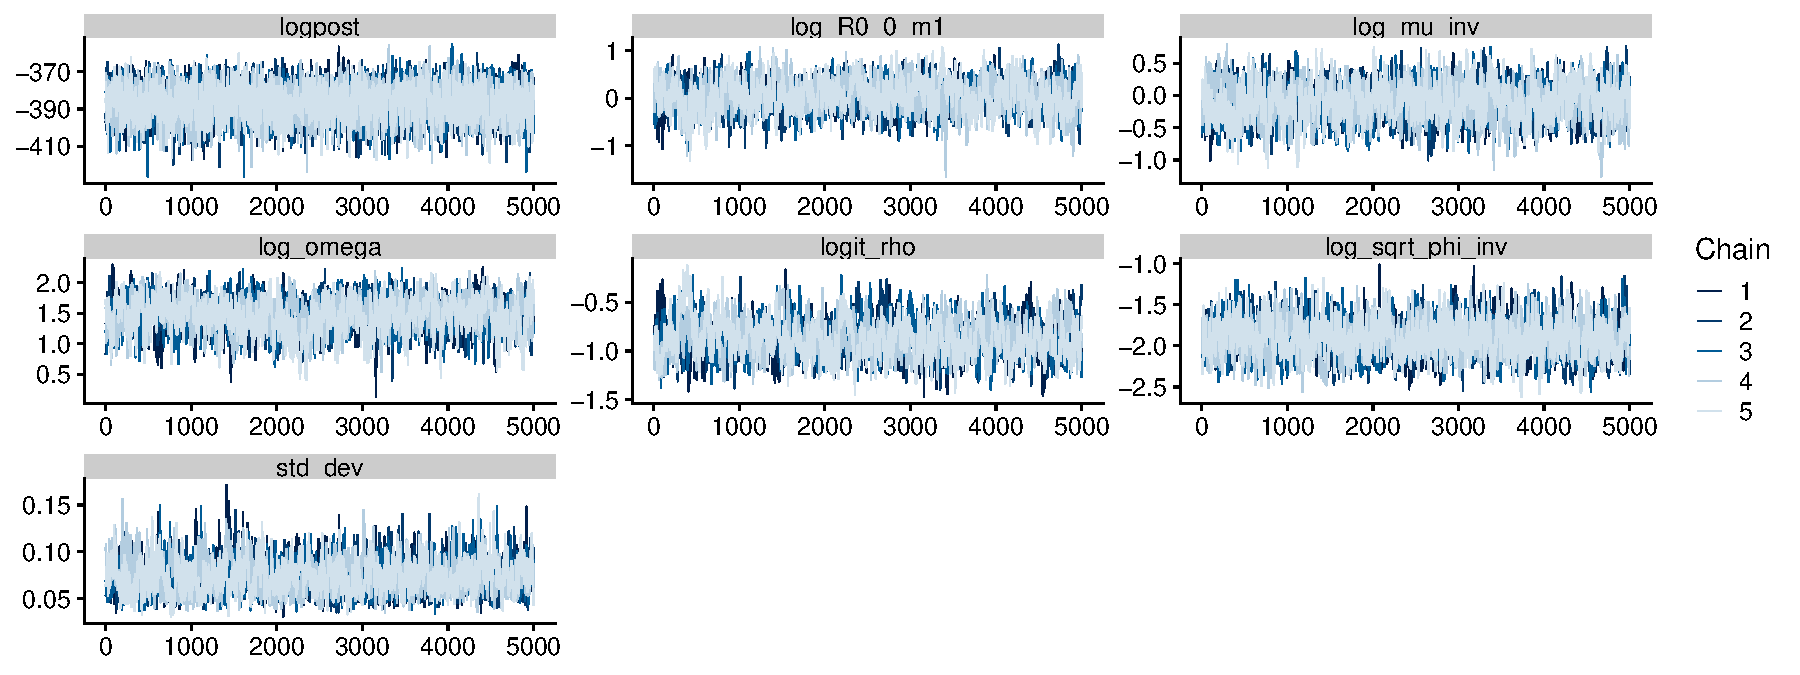
\includegraphics[width=\linewidth]{figures/sinfoi_rw1_traces}
	\caption{Posterior traceplots for SIRS model parameters with time--varying force of infection.}
	\label{fig:sinfoirw1traces}
\end{figure}

\begin{figure}[htbp]
	\centering
	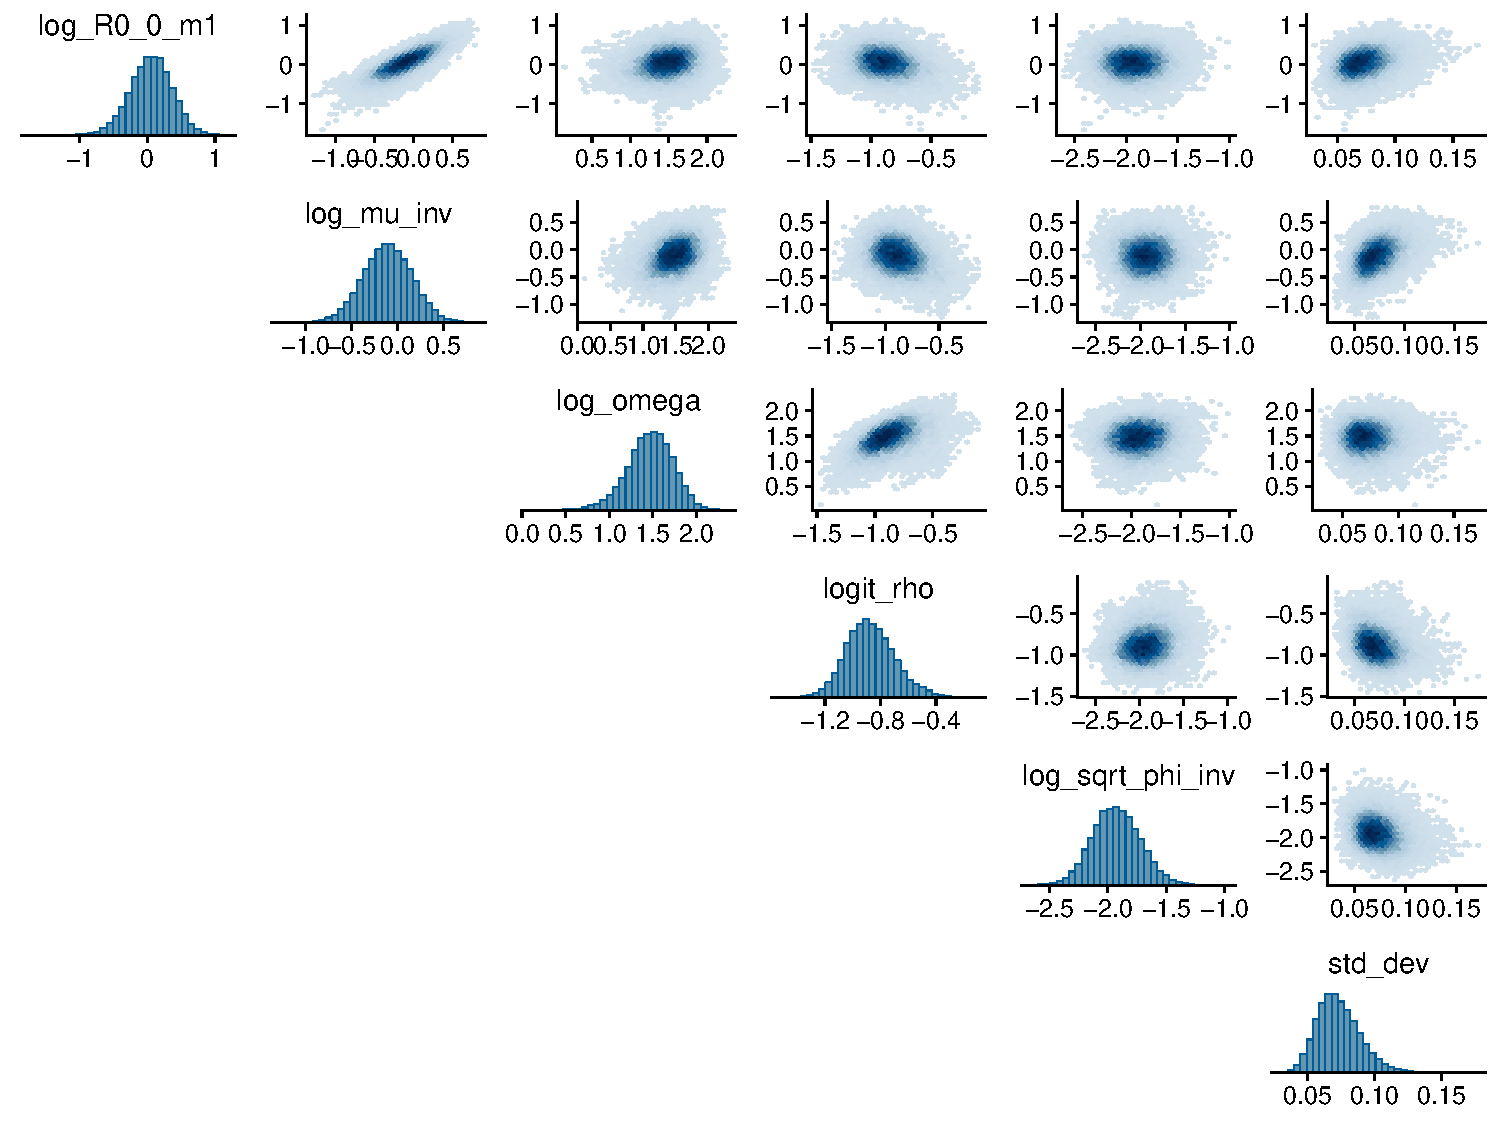
\includegraphics[width=\linewidth]{figures/sinfoi_rw1_pairs}
	\caption{Posterior histograms and pairwise hexplots for SIRS model parameters with time--varying force of infection.}
	\label{fig:sinfoirw1pairs}
\end{figure}

\begin{figure}[htbp]
	\centering
	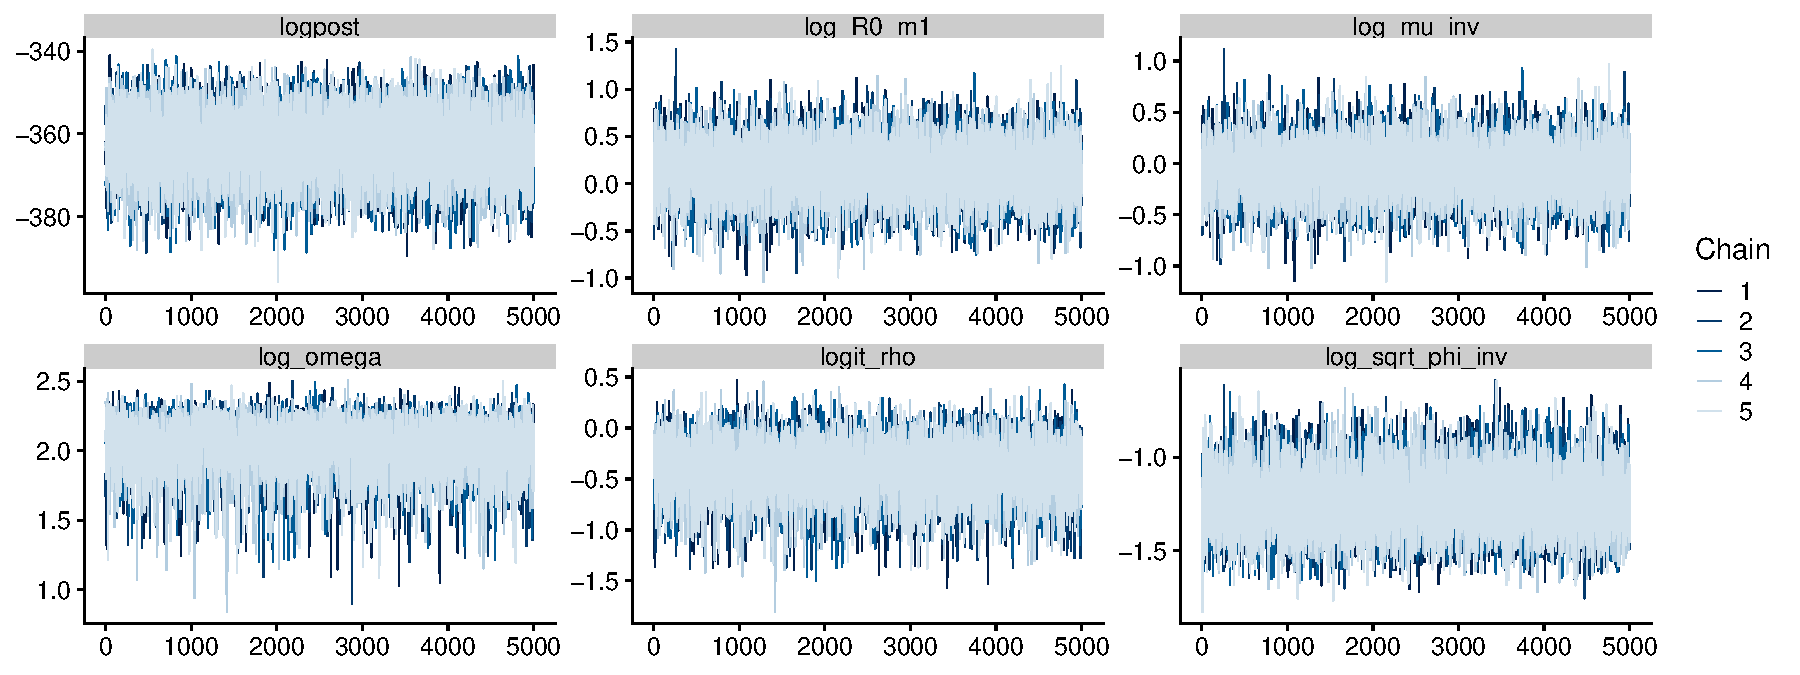
\includegraphics[width=\linewidth]{figures/sinfoi_const_traces}
	\caption{Posterior traceplots for SIRS model parameters with time--homogeneous force of infection.}
	\label{fig:sinfoiconsttraces}
\end{figure}

\begin{figure}[htbp]
	\centering
	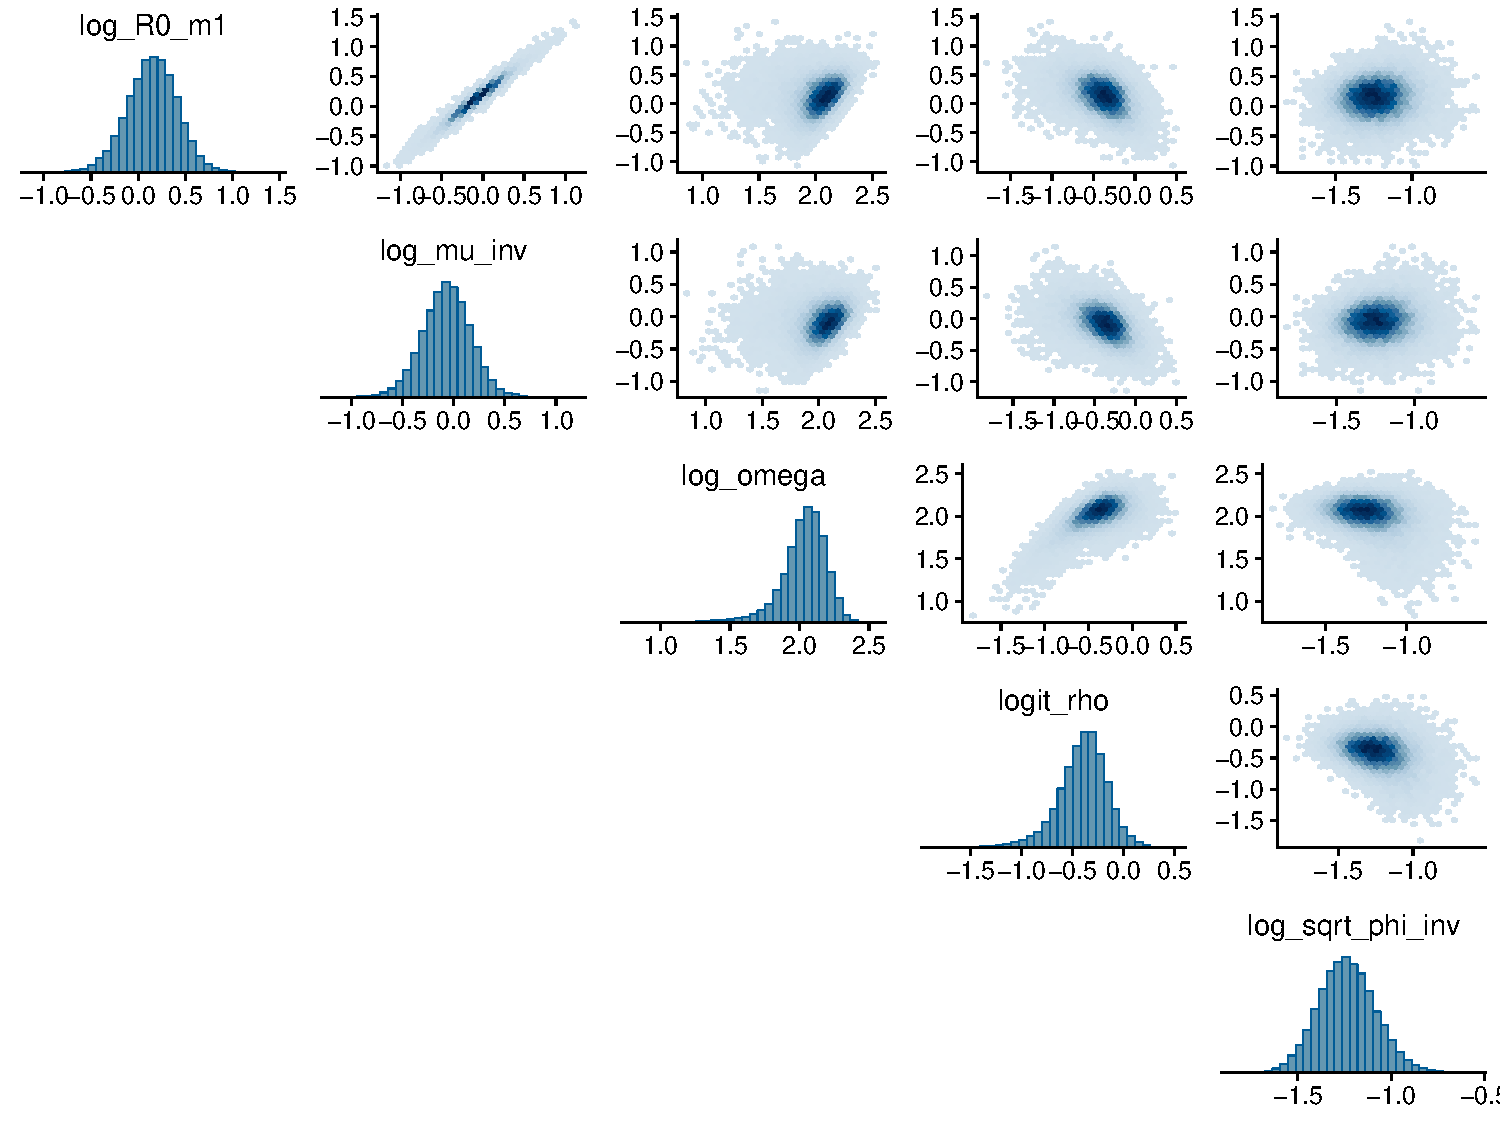
\includegraphics[width=\linewidth]{figures/sinfoi_const_pairs}
	\caption{Posterior histograms and pairwise hexplots for SIRS model parameters with time--homogeneous force of infection.}
	\label{fig:sinfoiconstpairs}
\end{figure}

\begin{figure}[htbp]
	\centering
	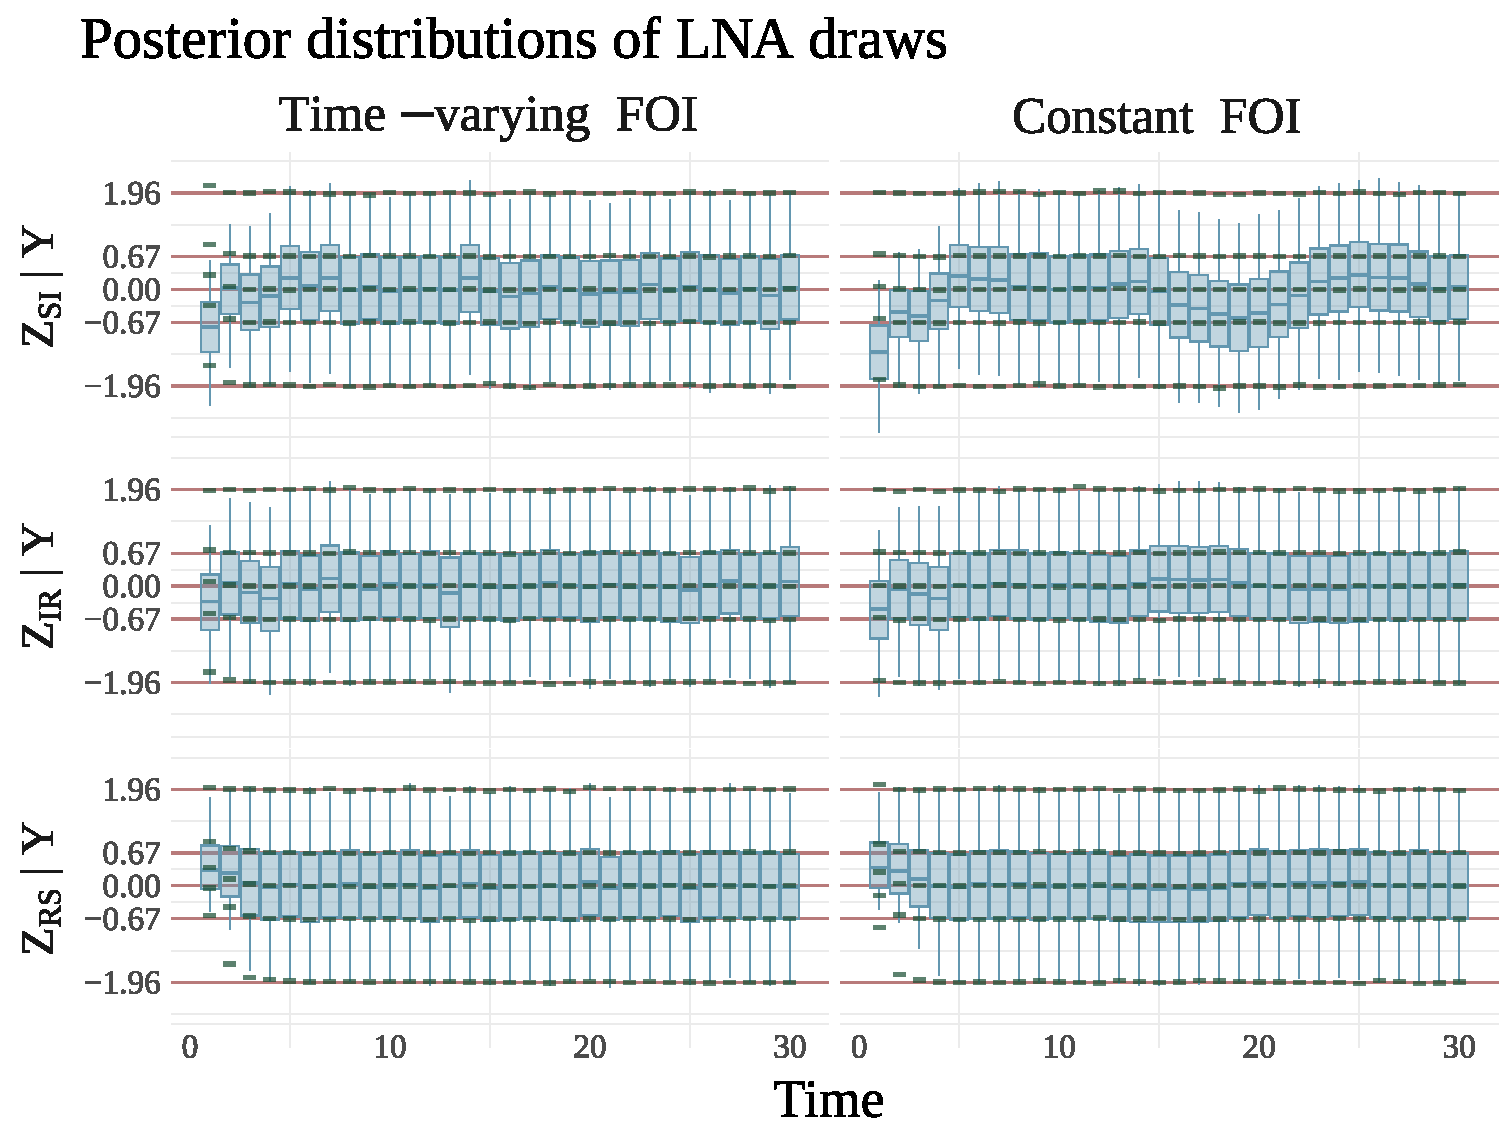
\includegraphics[width=\linewidth]{figures/sinfoi_lna_drawplots}
	\caption[Posterior distributions of LNA draws for SIRS models with time--varying and constant force of infection.]{Posterior distributions of the LNA draws for infection, recovery, and loss of immunity in SIRS models with time--varying and constant force of infection (blue boxplots). The lower and upper whisker tips correspond to the $ 2.5^\mr{th} $ and $ 97.5^\mr{th} $ posterior quantiles, the lower and upper hinges to the $ 25^\mr{th} $ and $ 75^\mr{th} $ quantiles, and the middle hash mark to the posterior median. The solid red lines are the theoretical quantiles of the posterior predictive distribution (or equivalently, the prior distribution) of the LNA draws, drawn at the quantiles of a standard normal distribution corresponding to the boxplot quantiles. The green ticks are the estimated quantiles of the posterior predictive distributions of the LNA draws, accounting for boundary conditions on the state space of the latent process and obtained by simulating LNA paths from the posterior predictive distribution. The posterior distributions of LNA draws are shaded according to the level of posterior shrinkage, computed as one minus the ratio of standard deviations of LNA draws in the posterior and prior.}
	\label{fig:sinfoidrawplots}
\end{figure}

\newpage
\section{Specification of Contact Rates}
\label{sec:flu_contact_rates}

Contact rates within and between age--strata were obtained from the Finnish arm of the POLYMOD survey \cite{mossong2008social,polymod}, and were accessed via the \texttt{socialmixr R} package \cite{funk2018socialmixr}. The survey was a population--based, prospective survey that recorded contact rates by sex, age, location, duration, and frequency. We queried the symmetric form of the estimated mean contact matrix aggregated age--strata in our analysis (0--19 years and 20+ years), which based on a sample of 1,006 individuals. A contact matrix is said to be symmetric if the total number of contacts between two groups is equal. In particular, if $ c_{ij} $ is the mean number of contacts an individual in group $ i $ has with members of group $ j $, and group $ i $ is of size $ N_i $, then symmetry requires that $ c_{ij}N_i = c_{ji}N_j $. Due to the vagaries of sampling variability, this relation does not always hold. The symmetric contact matrix is obtained by taking $ c_{ij}^{\prime} = (c_{ij}N_i + c_{ji}N_j) / 2N_i $. 

The estimated mean contact rates are
\[ \bC_{tot} = 
\kbordermatrix{
	 & 0-19 & 20+ \\
	 0-19 & 7.44 & 5.05 \\
	 20+ & 1.55 & 8.56
}. \]
Following \cite{meyer2017incorporating}, we row--normalize the matrix, thus removing differences in absolute contact rates. This is helpful in parameterizing and assigning sensible priors to other aspects of the model, such as basic reproduction numbers. The normalized contact rates are
\[ \bC = 
\kbordermatrix{
	& 0-19 & 20+ \\
	0-19 & 0.60 & 0.40 \\
	20+ & 0.15 & 0.85
}. \]

\newpage
\section{Mapping Standard Normal Draws to LNA Sample Paths with Forcings}
\label{sec:dolna_forcings}
\begin{algorithm}[htbp]
	\caption{Mapping standard normal draws onto LNA sample paths with forcings.}
	\label{alg:doLNA2}
	\begin{algorithmic}[1]
		\Procedure{doLNA2}{$ \bZ,\btheta,\mcI,\bxi $}
		\State \textbf{initialize: }$ \bX(t_0) \gets \bX_0,\ \bN(t_0) \gets \bs{0},\ \bNtil(t_0) \gets \bs{0},\ \bmu(t_0) \gets \bs{0},\ \bSigma(t_0) \gets \bs{0} $
		\For{$ \ell = 1,\dots,L $}
		\State $ \bmu(t_\ell),\ \bSigma(t_\ell) \gets $ solutions to (\ref{eqn:lna_ode_drift}) and (\ref{eqn:lna_ode_diffusion}) over $ (t_{\ell-1}, t_\ell] $
		\State $ \bNtil(t_\ell)\gets \bmu(t_\ell) + \bSigma(t_\ell)^{1/2}\bZ(t_\ell) $ \Comment{non--centered parameterization}
		\State $ \bN(t_\ell)\gets \bN(t_{\ell-1}) + \exp(\bNtil(t_\ell)) - \bs{1} $
		\State \textbf{restart initial conditions:} 
		  \vspace{-0.15in}\hspace{0.2in} \begin{align*}
			\bX(t_\ell) &\gets \bX(t_{\ell-1}) + \bA^T(\bN(t_\ell)-\bN(t_{\ell-1})) \\
			\bX(t_\ell^+) &\gets \bX(t_\ell) + \bxi(t_\ell)\\
			\bNtil(t_\ell) &\gets \bs{0},\ \bmu(t_\ell)\gets\bs{0},\ \bSigma(t_\ell)\gets\bs{0}
			\end{align*}\vspace{-0.35in}
		\EndFor
		\State \hspace{-0.25in}\Return \Comment{return incidence and/or prevalence sample paths}
		\State$\bN = \left \lbrace\bN(t_0),\bN(t_1),\dots,\bN(t_L)\right \rbrace,\ \bX = \left \lbrace \bX(t_0),\ \bX(t_1),\dots,\bX(t_\ell) \right \rbrace $
		\EndProcedure
	\end{algorithmic}
\end{algorithm}

\newpage
\section{Joint Sampling of LNA Paths and Gaussian Markov Random Fields}
\label{sec:lna_ess_gmrf}

Jointly sampling the LNA draws and the values of a GMRF, $ \bF $, in addition to possibly any other latent Gaussian parameters including the initial compartment volumes as in Section \ref{sec:lna_init_volumes}, requires trivially modifying Algorithm \ref{alg:elliptss_lna_initvols} to include the additional parameters. We implement the same computational strategy used throughout Chapters \ref{chap:lna_for_sems} and \ref{chap:lna_extensions} of using non--centered parameterizations for the parameters of interest and the LNA path. As we have noted, this has the advantage of breaking the autocorrelation that would otherwise lead to poor MCMC mixing when using a centered parameterization and alternating between updates to different parameters in the model. We will denote by $ \bZ = (\bZ^X,\ \bZ^{X_0},\ \bZ^F,\ \bZ^{\btheta_F}) $ the multivariate standard normal draws for the latent LNA process, the initial compartment volumes, the draws to be mapped to the GMRF, and $ \bZ^{\btheta_F} $ the draws that are mapped to the GMRF hyper--parameters that are to be updated along with the GMRF. Unless otherwise stated (and we never do so state), we will at the very least update the precision or standard deviation of the GMRF increments jointly with the field to avoid poor MCMC mixing. We will assume that non--centered parameterizations for the GMRF and the hyper--parameters are linear transformations and thus do not require Jacobian terms to be included in the ElliptSS acceptance probability. We will denote by $ \bm_0 $, $ \bm_\theta $, $ \bV_0 $, and $ \bV_\theta $ the means and covariance matrices of the initial volumes and hyper--parameters, and by $ \doGMRF $ the linear operator for mapping $ \bZ^F $ to a GMRF sample, i.e., the GMRF values are obtained by $ \doGMRF(\bZ^F; \btheta_F) $. 

\begin{algorithm}[htbp]
	\caption{Sampling LNA draws, initial volumes, GMRF values, and GMRF hyper--parameters via elliptical slice sampling.}
	\label{alg:elliptss_lna_gmrf}
	\begin{algorithmic}[1]
		\Procedure{\doElliptSS3}{$ \bZ = (\bZ^X_{cur}, \bZ^{X_0}_{cur},\bZ^{F},\bZ^{\btheta_F}),\btheta,\bY,\mcI,\omega = 2\pi $}
		\State Sample ellipse: $ \bZ_{prop} \sim N(\bs{0}, \mb{I})$
		\State Sample threshold: $ u|\bx \sim \mr{Unif}(0, L(\bY|\doLNA(\bZ_{cur},\btheta,\mcI))) $
		\State Position the bracket: \vspace{-0.15in}
		\begin{align*}
		\psi &\sim \mr{Unif}(0,\omega)\\
		L_\psi &\leftarrow -\psi;\ R_\psi \leftarrow L_\psi + \psi\\
		\phi &\sim \mr{Unif}(L_\psi,R_\psi)
		\end{align*}
		\State Compute the proposal: \vspace{-0.1in}\begin{align*}
		\bZ^\prime &\leftarrow \bZ_{cur}\cos(\phi) + \bZ_{prop}\sin(\phi) \\
		&\implies \bX_0^\prime = \bm_0 + \bV_0^{1/2}\bZ^{X_0^\prime}\\
		&\implies\btheta_F^\prime = \bm_\theta + \bV_\theta^{1/2}\bZ^{\theta_F^\prime} \\
		&\implies\bF^\prime = \doGMRF(\bZ^F;\btheta_F)
		\end{align*}
		\If{$ L(\bY|\doLNA(\bZ^{X\prime},\bX_0^\prime,\bF^\prime,\btheta_F^\prime,\btheta,\mcI)) > u $}{ accept $ \bZ^\prime $}
		\State\Return{ $ \bZ' $}
		\Else
		\State Shrink bracket and try a new angle:
		\State{\textbf{If:} $ \phi < 0 $}{ \textbf{then: }$ L_\phi \leftarrow\phi $ }{ \textbf{else: }$ R_\phi \leftarrow \phi $}
		\State $ \phi \sim \mr{Unif}(L_\phi, R_\phi) $
		\State \textbf{GoTo:} 5
		\EndIf
		\EndProcedure
	\end{algorithmic}
\end{algorithm}

\section{Modeling Pandemic A(H1N1) Influenza in Finland --- Additional Details and Supplementary Results}
\label{sec:flu_supplement}

\subsection{MCMC Details}
\label{subsec:flu_mcmc_details}
We fit age--vaccination stratified SIRS ODE models with time varying dynamics to pandemic A(H1N1) influenza incidence data. The vaccination adjusted reproduction numbers were modeled using either a GMRF or as piecewise homogeneous within three epochs. The models were fit using the same prior regimes, given in Table \ref{tab:flu_priors}. We ran five chains for each model, initialized at random parameter values, for 100,000 iterations per chain. Model parameters (excluding noncentered GMRF draws and hyperparameters, as described in Section \ref{subsec:flu_mcmc}) were jointly updated via MVNSS (see Section \ref{subsubsec:mvn_slice_sampling}). The empirical covariance for the MVNSS algorithm was adapted over the first 50,000 iterations using the gain factor sequence, $\gamma_n = 0.5(1 + 0.01n)^{-0.9}$. The contribution of isotropic Gaussian noise to the proposal was initialized at 0.001 and reduced throughout the adaptation phase according to the sequence $ \iota_n = 0.001(1 + 0.01n)^{-0.99} $. In the GMRF model, the non--centered GMRF draws were updated via ElliptSS along with their hyperparameters, hence MCMC alternated between one ElliptSS and one MVNSS update per MCMC iteration. The ElliptSS bracket width was reset after the first 5,000 MCMC iterations to $ \omega = 2\sqrt{2\log(10)}\sigma_{ElliptSS}$, where $ \sigma_{ElliptSS} $ was the standard deviation of the accepted angles over the initial iterations. The MCMC estimation scales for the non--GMRF parameters were parameterized as in Table \ref{tab:flu_params_est}, and the GMRF was parameterized using the NCP given in Section \ref{subsec:flu_gmrf}. Convergence was assessed visually by inspection of traceplots of posterior samples. The models took between roughly one hour to run.

\newpage
\subsection{Prior Specification}
\label{subsec:flu_priors}

\subsubsection{Priors for effective population sizes}
\label{subsubsec:flu_effpop_priors}

At the start of the modeling period, individuals in the population were assigned to either be susceptible or detached from the transmission process. The fraction of the population that was susceptible defines the effective population size. We identify the scale of the prior for the susceptible fraction of the population by inflating the total number of cases that were detected in each season by the case detection rate and the fraction of the effective population size that we would expect to be infected in a deterministic outbreak with SIR dynamics over a reasonable range of basic reproduction numbers. We ignored age structure for the sake of simplicity and assumed that the same fraction of youths and adults were initially susceptible. Results from a sensitivity analysis in which we assumed that a larger fraction of youths were initially susceptible are presented in Section \ref{subsec:flu_highsusc_sensitivity}.

The final size relation for the SIR model \cite{miller2012note} relates the fraction of the population that is infected under SIR dynamics, $ \pi $, to the basic reproduction number via: 
$$(1-\pi) = \exp^{-\pi R_0}.$$
Roughly 10,000 cases were detected in all age groups over the course of both seasons. If the reproduction numbers and detection rates were stable across seasons, which might not be unreasonable if the lower attack rate in the second season is the result of depletion of susceptibles in the first season, a very crude estimate of the number of susceptibles is $$\what{s} = \frac{10000}{\rho(1-\pi)},$$
where $ \rho $ is the detection rate. Hence, the fraction of the population that is in the susceptible compartment is $ \what{s}N $. Effective population sizes for different reproduction numbers that are typical of A(H1N1)pdm09 \cite{biggerstaff2014estimates} and detection rates \cite{shubin2016revealing} are given in Table \ref{tab:flu_effpop_priors}. 

In the main analysis presented in Section \ref{sec:flu_results}, we used a multivariate normal approximation to a dirichlet--multinomial distribution for the initial distribution of individuals of each age stratum. The hyperparameter, $$ \balpha_j = ({S_{j,0}^{(u)}} = 25, {I_{j,0}^{(u)}}=0,{R_{j,0}^{(u)}}=0,D_{j,0}^{(v)} = 75), $$ was centered so that 25\% of each stratum was initially susceptible, with the central 80\% of the prior mass between 20\% and 30\%. 

\begin{table}[htbp]
	\caption{Effective fraction of the population that is susceptible for different reproduction numbers and dection rates.}
	\label{tab:flu_effpop_priors}
	\centering
	\begin{tabular}{lcccc}
		& \multicolumn{4}{c}{\textbf{Detection rate} ($ \rho $)}\\
		\cmidrule{2-5}$ \mb{R_0} $&  0.0075 & 0.01 & 0.015 &0.02\\
		\hline
		1.25 & 0.40 & 0.30 & 0.20 & 0.15\\
		1.5 & 0.60 & 0.45 & 0.30 & 0.22\\
		1.75 & 0.87 & 0.65 & 0.43 & 0.33\\
		\hline
	\end{tabular}
\end{table}

\subsubsection{Priors for time--homogeneous parameters}
\label{subsubsec:flu_param_priors_homog}

\begin{sidewaystable}[htbp]
	\begin{fullpage}
		\caption[Parameters and priors for age--vaccination stratified SIRS ODE models fit to the A(H1N1)pdm09 influenza outbreak in Finland.]{Parameters and priors for age--vaccination stratified SIRS ODE models fit to the A(H1N1)pdm09 influenza outbreak in Finland, prior distributions used in the main analysis. Vaccination adjusted intrinsic reproduction numbers are defined as in equation (\ref{eqn:R0_adj}). The form of the parameter listed in the leftmost column corresponds to the estimation scale used in the MCMC. All parameters in this table were jointly updated using multivariate normal slice sampling.}
		\label{tab:flu_priors}
		\scriptsize
		\centering
		\begin{tabular}{lllrr}
			\hline
			\textbf{Param.} &  \textbf{Interpretation} & \textbf{Prior} & \textbf{Median (90\% Interval)} & \textbf{References/Justification} \\ \hline
			$ \log(\psi_{Y,0}) $ & Intrinsic reproduction \# & $N$(log(1.1), $ 0.06^2 $) & $ \psi^{adj}_{Y,0} = 1.10\ (1.00, 1.21) $ & Nearly endemic dynamics \\ 
			$ \log(\psi_{Y,19}) $ & Intrinsic reproduction \# & $N$(log(1.5), $ 0.175^2 $) & $ \psi_{Y,19} = 1.50\ (1.12, 2.00) $ & \cite{biggerstaff2014estimates} \\ 
			$ \log(\psi^{adj}_{Y,71}) $ & Adjusted intrinsic reproduction \# & $N$(log(1.3), $ 0.11^2 $) & $ \psi^{adj}_{Y,71} = 1.3\ (1.08, 1.56) $ & \cite{biggerstaff2014estimates} and  $ \psi^{adj}_{Y,71} < \psi^{adj}_{A,71} $ \\ 
			$ \log(\psi^{adj}_{A,0}) $ & Intrinsic reproduction \# & $N$(log(1.05), $ 0.025^2 $) & $ \psi^{adj}_{A,0} = 1.10\ (1.00, 1.21) $ & Nearly endemic dynamics \\ 
			$ \log(\psi^{adj}_{A,19}) $ & Intrinsic reproduction \# & $N$(log(1.3), $ 0.11^2 $) & $ \psi^{adj}_{A,19} = 1.3\ (1.10, 1.78) $ & \cite{biggerstaff2014estimates} and$ \psi^{adj}_{A,19} < \psi^{adj}_{Y,19} $ \\ 
			$ \log(\psi^{adj}_{A,71}) $ & Adjusted intrinsic reproduction \# & $N$(log(1.4), $ 0.145^2 $) & $ \psi^{adj}_{A,71}= 1.4\ (1.10, 1.78) $ & \cite{biggerstaff2014estimates} and $ \psi^{adj}_{A,71} > \psi^{adj}_{Y,71} $ \\
			$ \log(\alpha_{Y,0}N_Ys_y) $ & Scaled rate of exogenous infection & $ N $(1.8, $ 0.54^2 $) & 6.0 (2.5, 14.7) & Small w.r.t. $ s_YN_Y $ \\ 
			$ \log(\alpha_{Y,19}\alpha_{Y,0}N_Ys_Y) $ & Scaled rate of exogenous infection& $ N $(2.3, $ 0.54^2 $) & 10.0 (4.1, 24.2) & Small w.r.t. $ s_YN_Y $ \\
			$ \log(\alpha_{Y,71}\alpha_{Y,0}N_Ys_Y) $ &Scaled rate of exogenous infection& $ N $(1.6, $ 0.54^2 $) & 5.0 (2.0, 12.0) & Small w.r.t. $ s_YN_Y $\\
			$ \log(\alpha_{A,0}\alpha_{A,0}N_As_A) $ & Scaled rate of exogenous infection & $ N $(3, $ 0.54^2 $) & 20 (8.2, 48.8) & Small w.r.t. $ s_AN_A $\\ 
			$ \log(\alpha_{A,19}N_As_A) $ & Scaled rate of exogenous infection& $ N $(3.2, $ 0.54^2 $) & 24.5 (10.1, 59.6) & Small w.r.t. $ s_AN_A $\\
			$ \log(\alpha_{A,71}N_as_A) $ & $ N $(2, $ 0.54^2 $) & Scaled rate of exogenous infection&  7.4 (3.0, 18.0) & Small w.r.t. $ s_AN_A $ \\
			$ 7/\mu_{Y}-1 $ & Avg. infectious period, youths (days--1) & $N$(0.41, 0.32$ ^2 $) & $  7/\mu_Y =$ 2.5 (1.9, 3.55) & \cite{biggerstaff2014estimates,carrat2008time,cori2012estimating,vink2014serial}\\
			$ 7/\mu_A -1 $ & Avg. infectious period, adults (days--1) & $N$(0.22, 0.165$ ^2 $) & $ 7/\mu_A =$ 2.25 (1.95, 2.63) & $ 1/\mu_Y > 1/\mu_A $,  \cite{biggerstaff2014estimates,carrat2008time,cori2012estimating,vink2014serial}\\
			$ \log(52/\omega) $ & Mean duration of immunity (years) & $N$(1.1, 0.3$ ^2 $) & $ 52/\omega = 3 $ (1.8, 4.9) & $ \Pr(\text{Lose immunity in 1 year}) = 0.3 $ \\
			$ \logit(\nu) $ & 1 - VE for susceptibility & $N$(-1.39, 1) & $ \nu = 0.2\ (0.05,\ 0.56) $ & \cite{lansbury2017effectiveness,syrjanen2014effectiveness}\\
			$ \logit(\rho_Y) $ & Mean case detection rate, youths & $ N(\logit(0.0125),\ 0.31^2) $& $ \rho = 0.0125\ (0.0075,\ 0.02) $ & \cite{shubin2016revealing}\\
			$ \logit(\rho_A) $ & Mean case detection rate, adults & $ N(\logit(0.01),\ 0.31^2) $& $ \rho = 0.01\ (0.006,\ 0.017) $ & $ \rho_A < \rho_Y $, \cite{shubin2016revealing}\\
			$ \log(1/\sqrt{\phi_Y}) $ & Neg. binom. overdispersion, youths & $ \exp(1) $ & 0.69 (0.05, 3.0) & It works.\\
			$ \log(1/\sqrt{\phi_A}) $ & Neg. binom. overdispersion, adults & $ \exp(1) $ & 0.69 (0.05, 3.0) & It works.\\
			\hline
		\end{tabular}
	\end{fullpage}
\end{sidewaystable}

\subsubsection{Priors for GMRFs}
\label{subsubsec:flu_gmrf_priors}

\begin{table}
	\caption[Priors for initial values of GMRFs for the numbers of exogenous infection in each age stratum.]{Priors for initial values of GMRFs for the numbers of exogenous infection in each age stratum. Parameters are subscripted by age stratum and week number, indexed from epiweek 15, 2009.}
	\label{tab:flu_alpha_gmrf_initpriors}
	\centering
	\begin{tabular}{lrr}
		\hline
		\textbf{Parameter} & \textbf{Prior} & \textbf{Median (90\% Interval)} \\ 
		$ \log(\alpha_{Y,0}) $ & $ N $(1.8, $ 0.54^2 $) & 6.0 (2.5, 14.7) \\ 
		$ \log(\alpha_{Y,19}) $ & $ N $(2.3, $ 0.54^2 $) & 10.0 (4.1, 24.2) \\
		$ \log(\alpha_{Y,71}) $ & $ N $(1.6, $ 0.54^2 $) & 5.0 (2.0, 12.0) \\
		$ \log(\alpha_{A,0}) $ & $ N $(3, $ 0.54^2 $) & 20 (8.2, 48.8) \\ 
		$ \log(\alpha_{A,19}) $ & $ N $(3.2, $ 0.54^2 $) & 24.5 (10.1, 59.6) \\
		$ \log(\alpha_{A,71}) $ & $ N $(2, $ 0.54^2 $) & 7.4 (3.0, 18.0) \\
		\hline
	\end{tabular}
\end{table}

\begin{table}
	\caption[Priors for standard deviations of GMRF increments of reproduction numbers and rates of exogenous infection.]{Priors for standard deviations of GMRF increments of reproduction numbers and rates of exogenous infection. Parameters are superscripted by whether they apply to a GRMF for intrinsic reproduction numbers, $ \psi $, or for numbers of exogenous infections, $ \alpha $, and are subscripted by age stratum and week number, indexed from epiweek 15, 2009.}
	\label{key}
	\centering
	\begin{tabular}{lrr}
		\hline
		\textbf{Parameter} & \textbf{Prior} & \textbf{Median (90\% Interval)} \\ 
		\hline
		$ \log(\sigma^{\psi}_{Y,0}) $ & $ N(-5.25, 0.125^2) $ & 0.0052 (0.0043, 0.0064)\\
		$ \log(\sigma^{\psi}_{Y,19}) $ & $ N(-4, 0.125^2) $ & 0.018 (0.015, 0.022)\\
		$ \log(\sigma^{\psi}_{Y,71}) $ & $ N(-5.25, 0.125^2) $ & 0.014 (0.012, 0.018)\\
		$ \log(\sigma^{\psi}_{A,0}) $ & $ N(-5.25, 0.125^2) $ & 0.0052 (0.0043, 0.0064)\\
		$ \log(\sigma^{\psi}_{A,19}) $ & $ N(-3.75, 0.125^2) $ & 0.024 (0.019, 0.029)\\
		$ \log(\sigma^{\psi}_{A,71}) $ & $ N(-5.25, 0.125^2) $ & 0.014 (0.012, 0.018)\\
		$ \log(\sigma^{\alpha}_{Y,0}) $ & $ N(-4.25, 0.25^2) $ & 0.014 (0.0095, 0.022)\\
		$ \log(\sigma^{\alpha}_{Y,19}) $ & $ N(-3.75, 0.25^2) $ & 0.024 (0.016, 0.035)\\
		$ \log(\sigma^{\alpha}_{A,71}) $ & $ N(-4, 0.25^2) $ & 0.018 (0.012, 0.028)\\
			$ \log(\sigma^{\alpha}_{Y,0}) $ & $ N(-4.25, 0.25^2) $ & 0.014 (0.0095, 0.022)\\
		$ \log(\sigma^{\alpha}_{A,19}) $ & $ N(-3.75, 0.25^2) $ & 0.024 (0.016, 0.035)\\
		$ \log(\sigma^{\alpha}_{A,71}) $ & $ N(-4, 0.25^2) $ & 0.018 (0.012, 0.028)\\
		\hline
	\end{tabular}
\end{table}

\begin{figure}
	\centering
	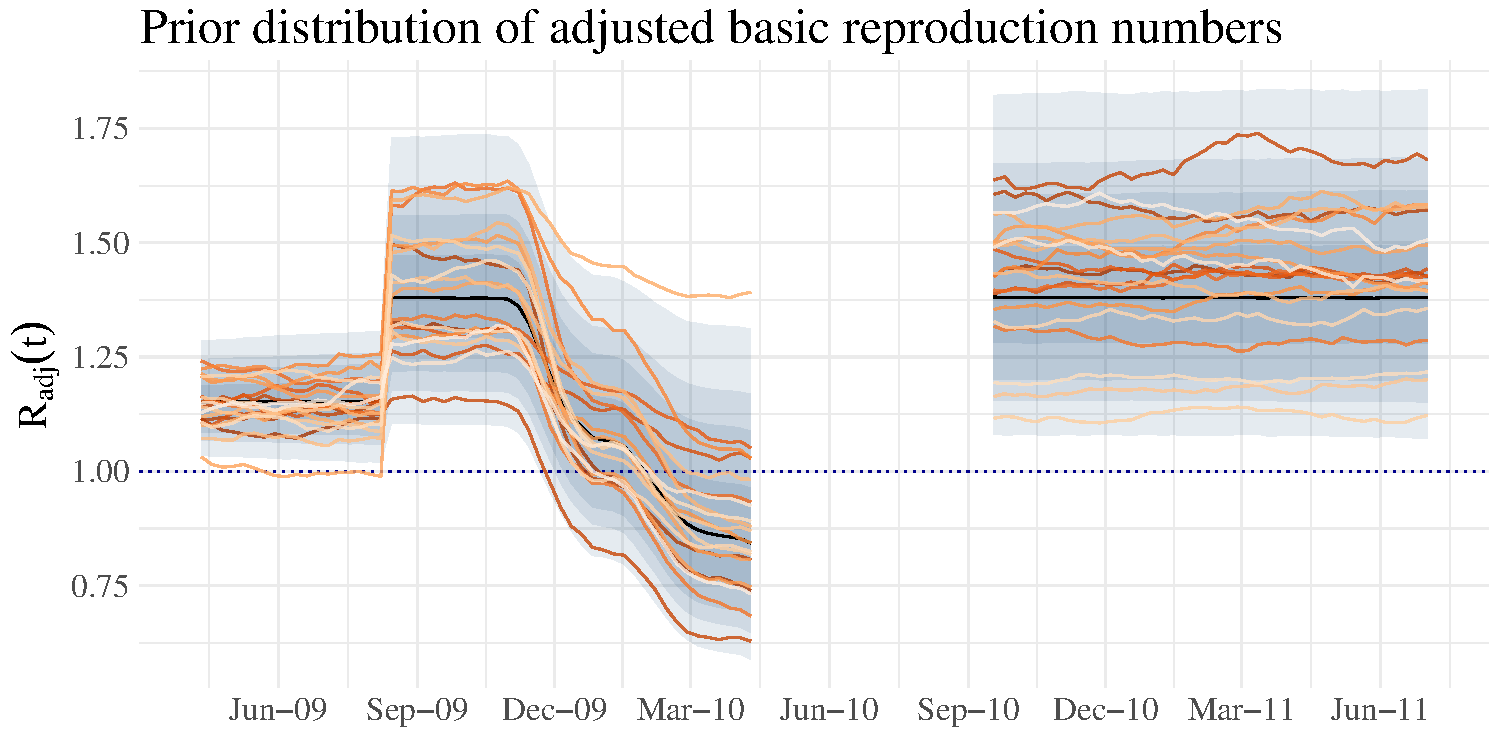
\includegraphics[width=\linewidth]{figures/flu_RW1_prior}
	\caption[Induced prior distribution of for vaccination adjusted basic reproduction numbers A(H1N1)pdm09 influenza in Finland.]{Induced prior distribution of for vaccination adjusted basic reproduction numbers A(H1N1)pdm09 influenza in Finland. Shaded bands correspond to the central 50\%, 80\%, and 95\% prior probability intervals. }
	\label{fig:flurw1prior}
\end{figure}

\begin{figure}
	\centering
	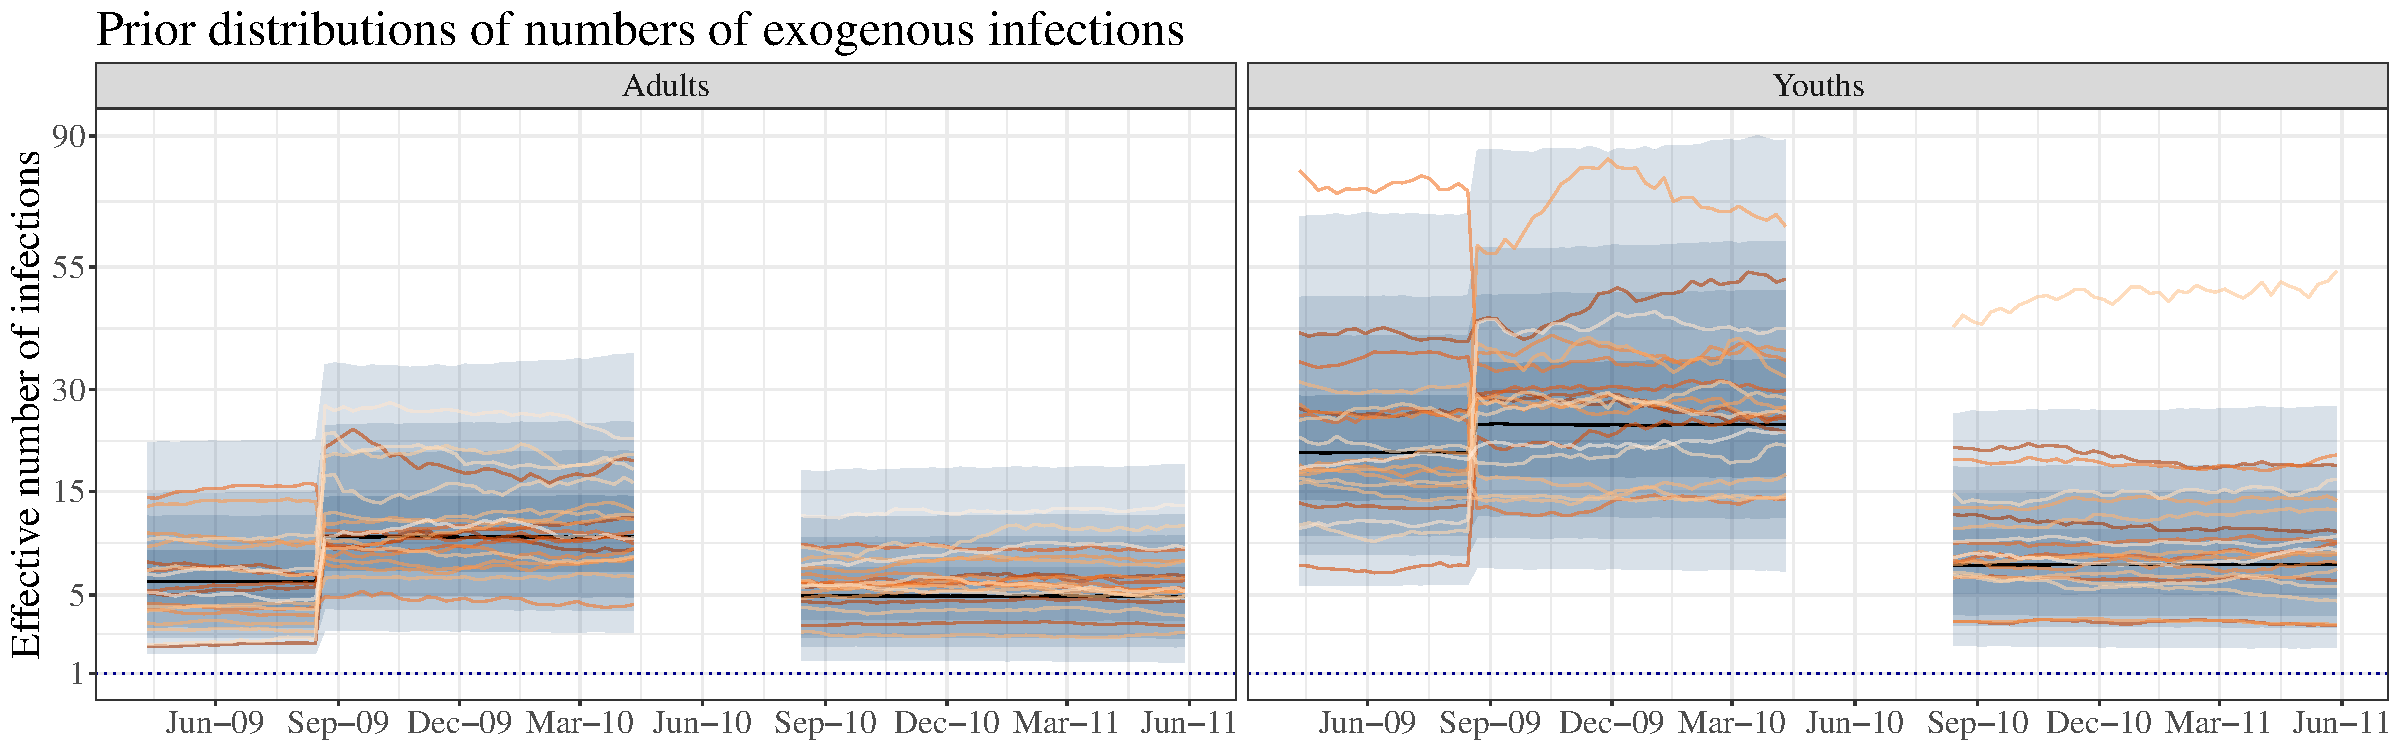
\includegraphics[width=\linewidth]{figures/flu_alpha_t_prior}
	\caption[Induced prior distribution of for effective numbers of exogenous infections among youths and adults.]{Induced prior distribution of for the effective number of exogenous infections among youths and adults. Shaded bands correspond to the central 50\%, 80\%, and 95\% prior probability intervals. }
	\label{fig:flualphaprior}
\end{figure}

\subsection{Additional Results}
\label{subsec:flu_additional_results}

\subsubsection{Stratified SIRS model with time--varying dynamics}
\label{subsubsec:flu_additional_res_rw1}

\begin{sidewaysfigure}[htbp]
	\centering
	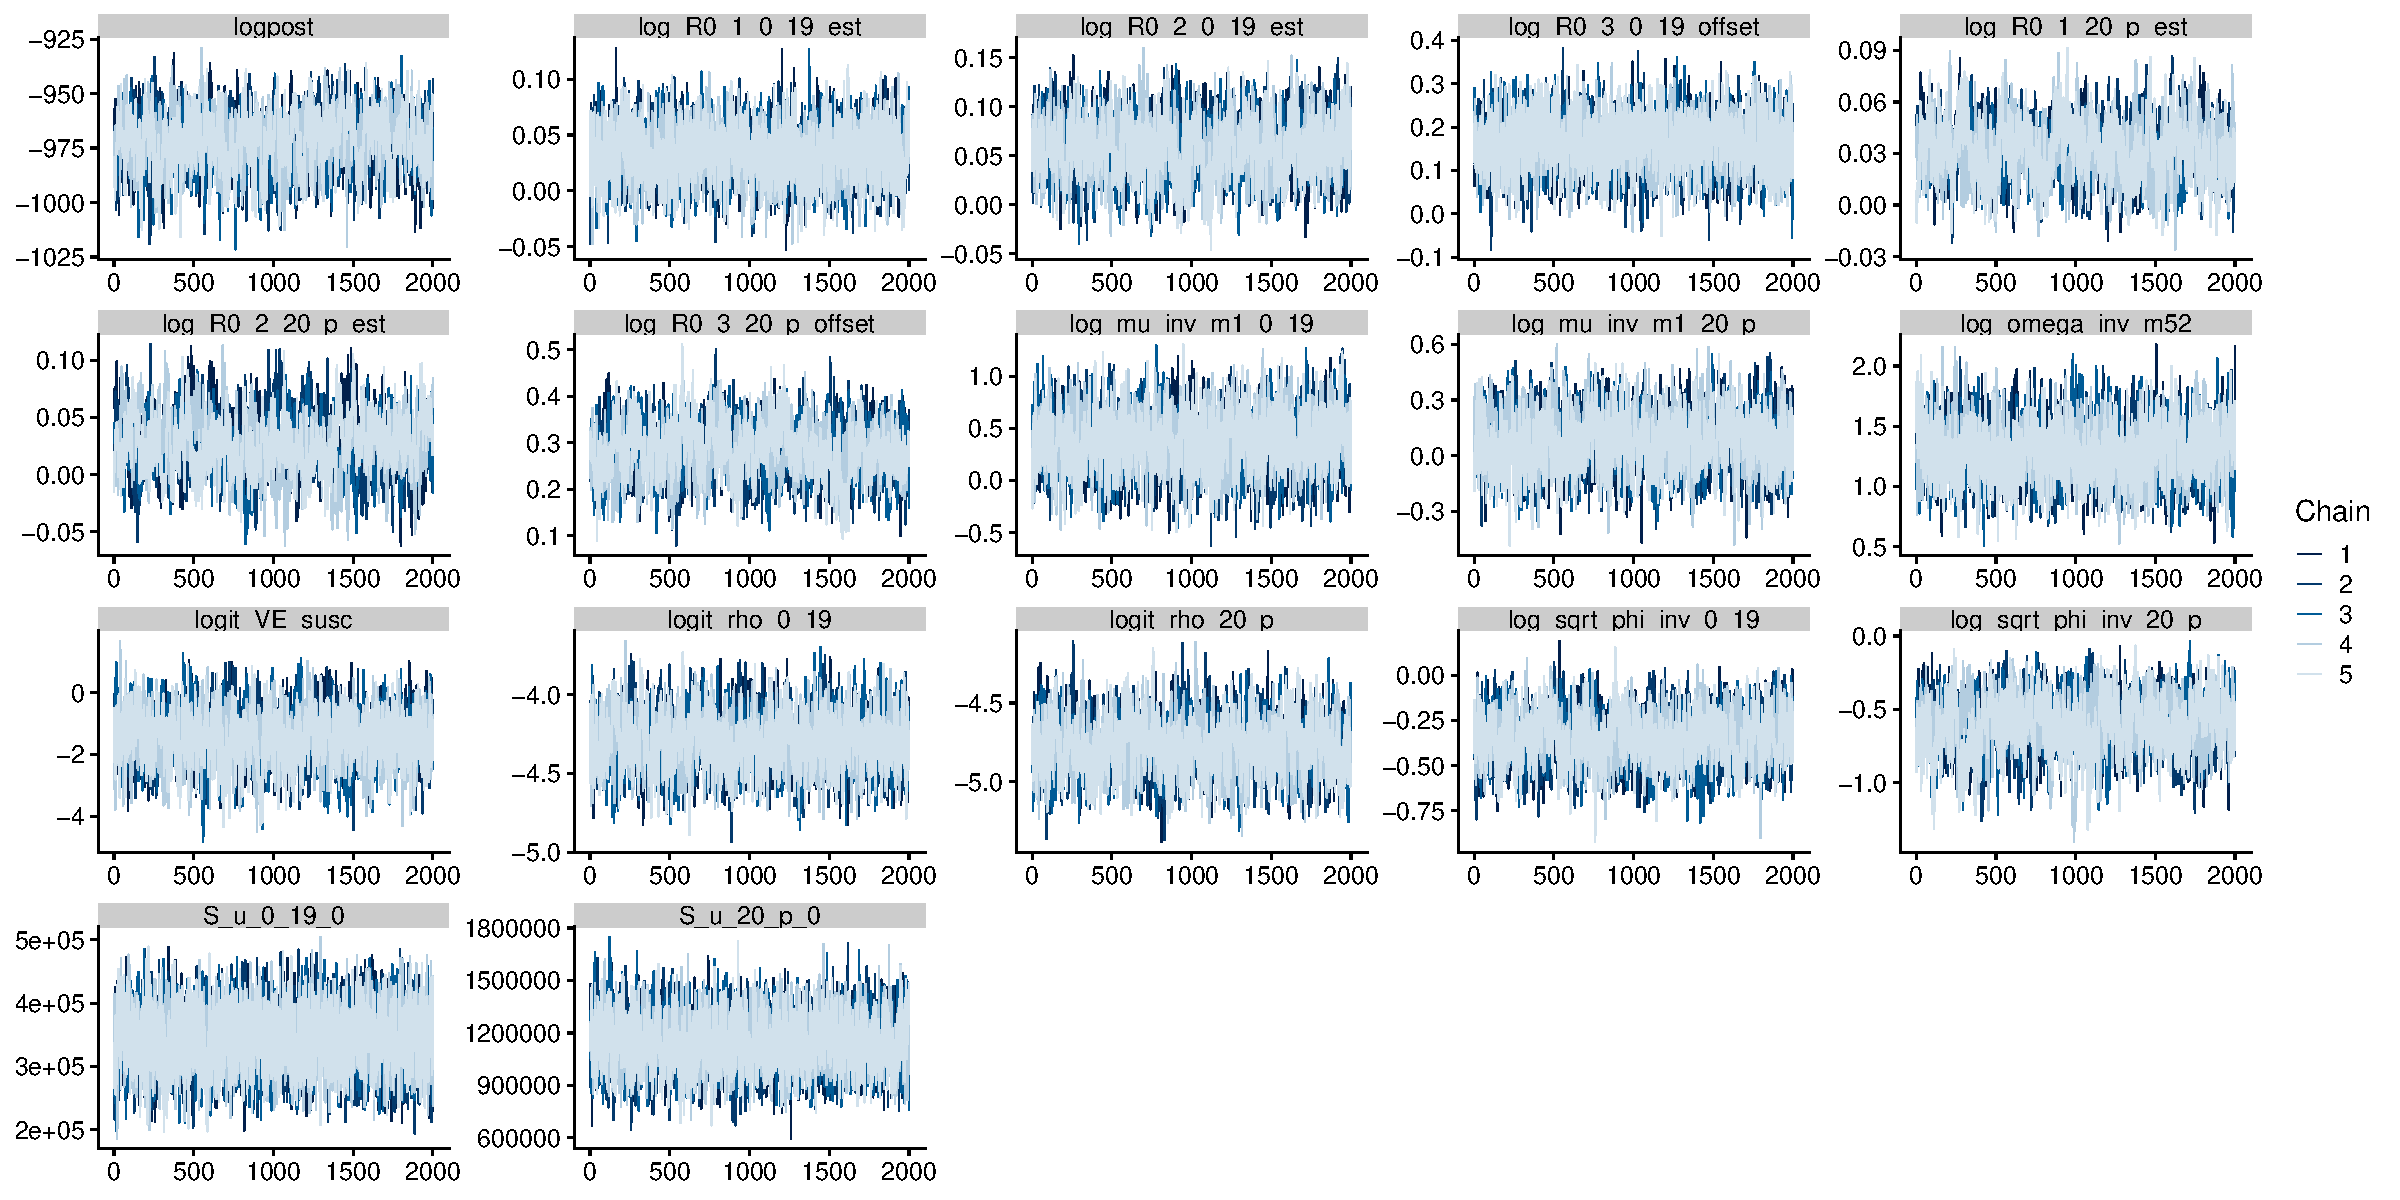
\includegraphics[width=\linewidth]{figures/flu_traces_rw_ode}
	\caption{Posterior traceplots for a stratified SIRS ODE model with time--varying dynamics fit to data from the A(H1N1) influenza pandemic in Finland.}
	\label{fig:flutracesrwode}
\end{sidewaysfigure}

\begin{sidewaysfigure}[htbp]
	\centering
	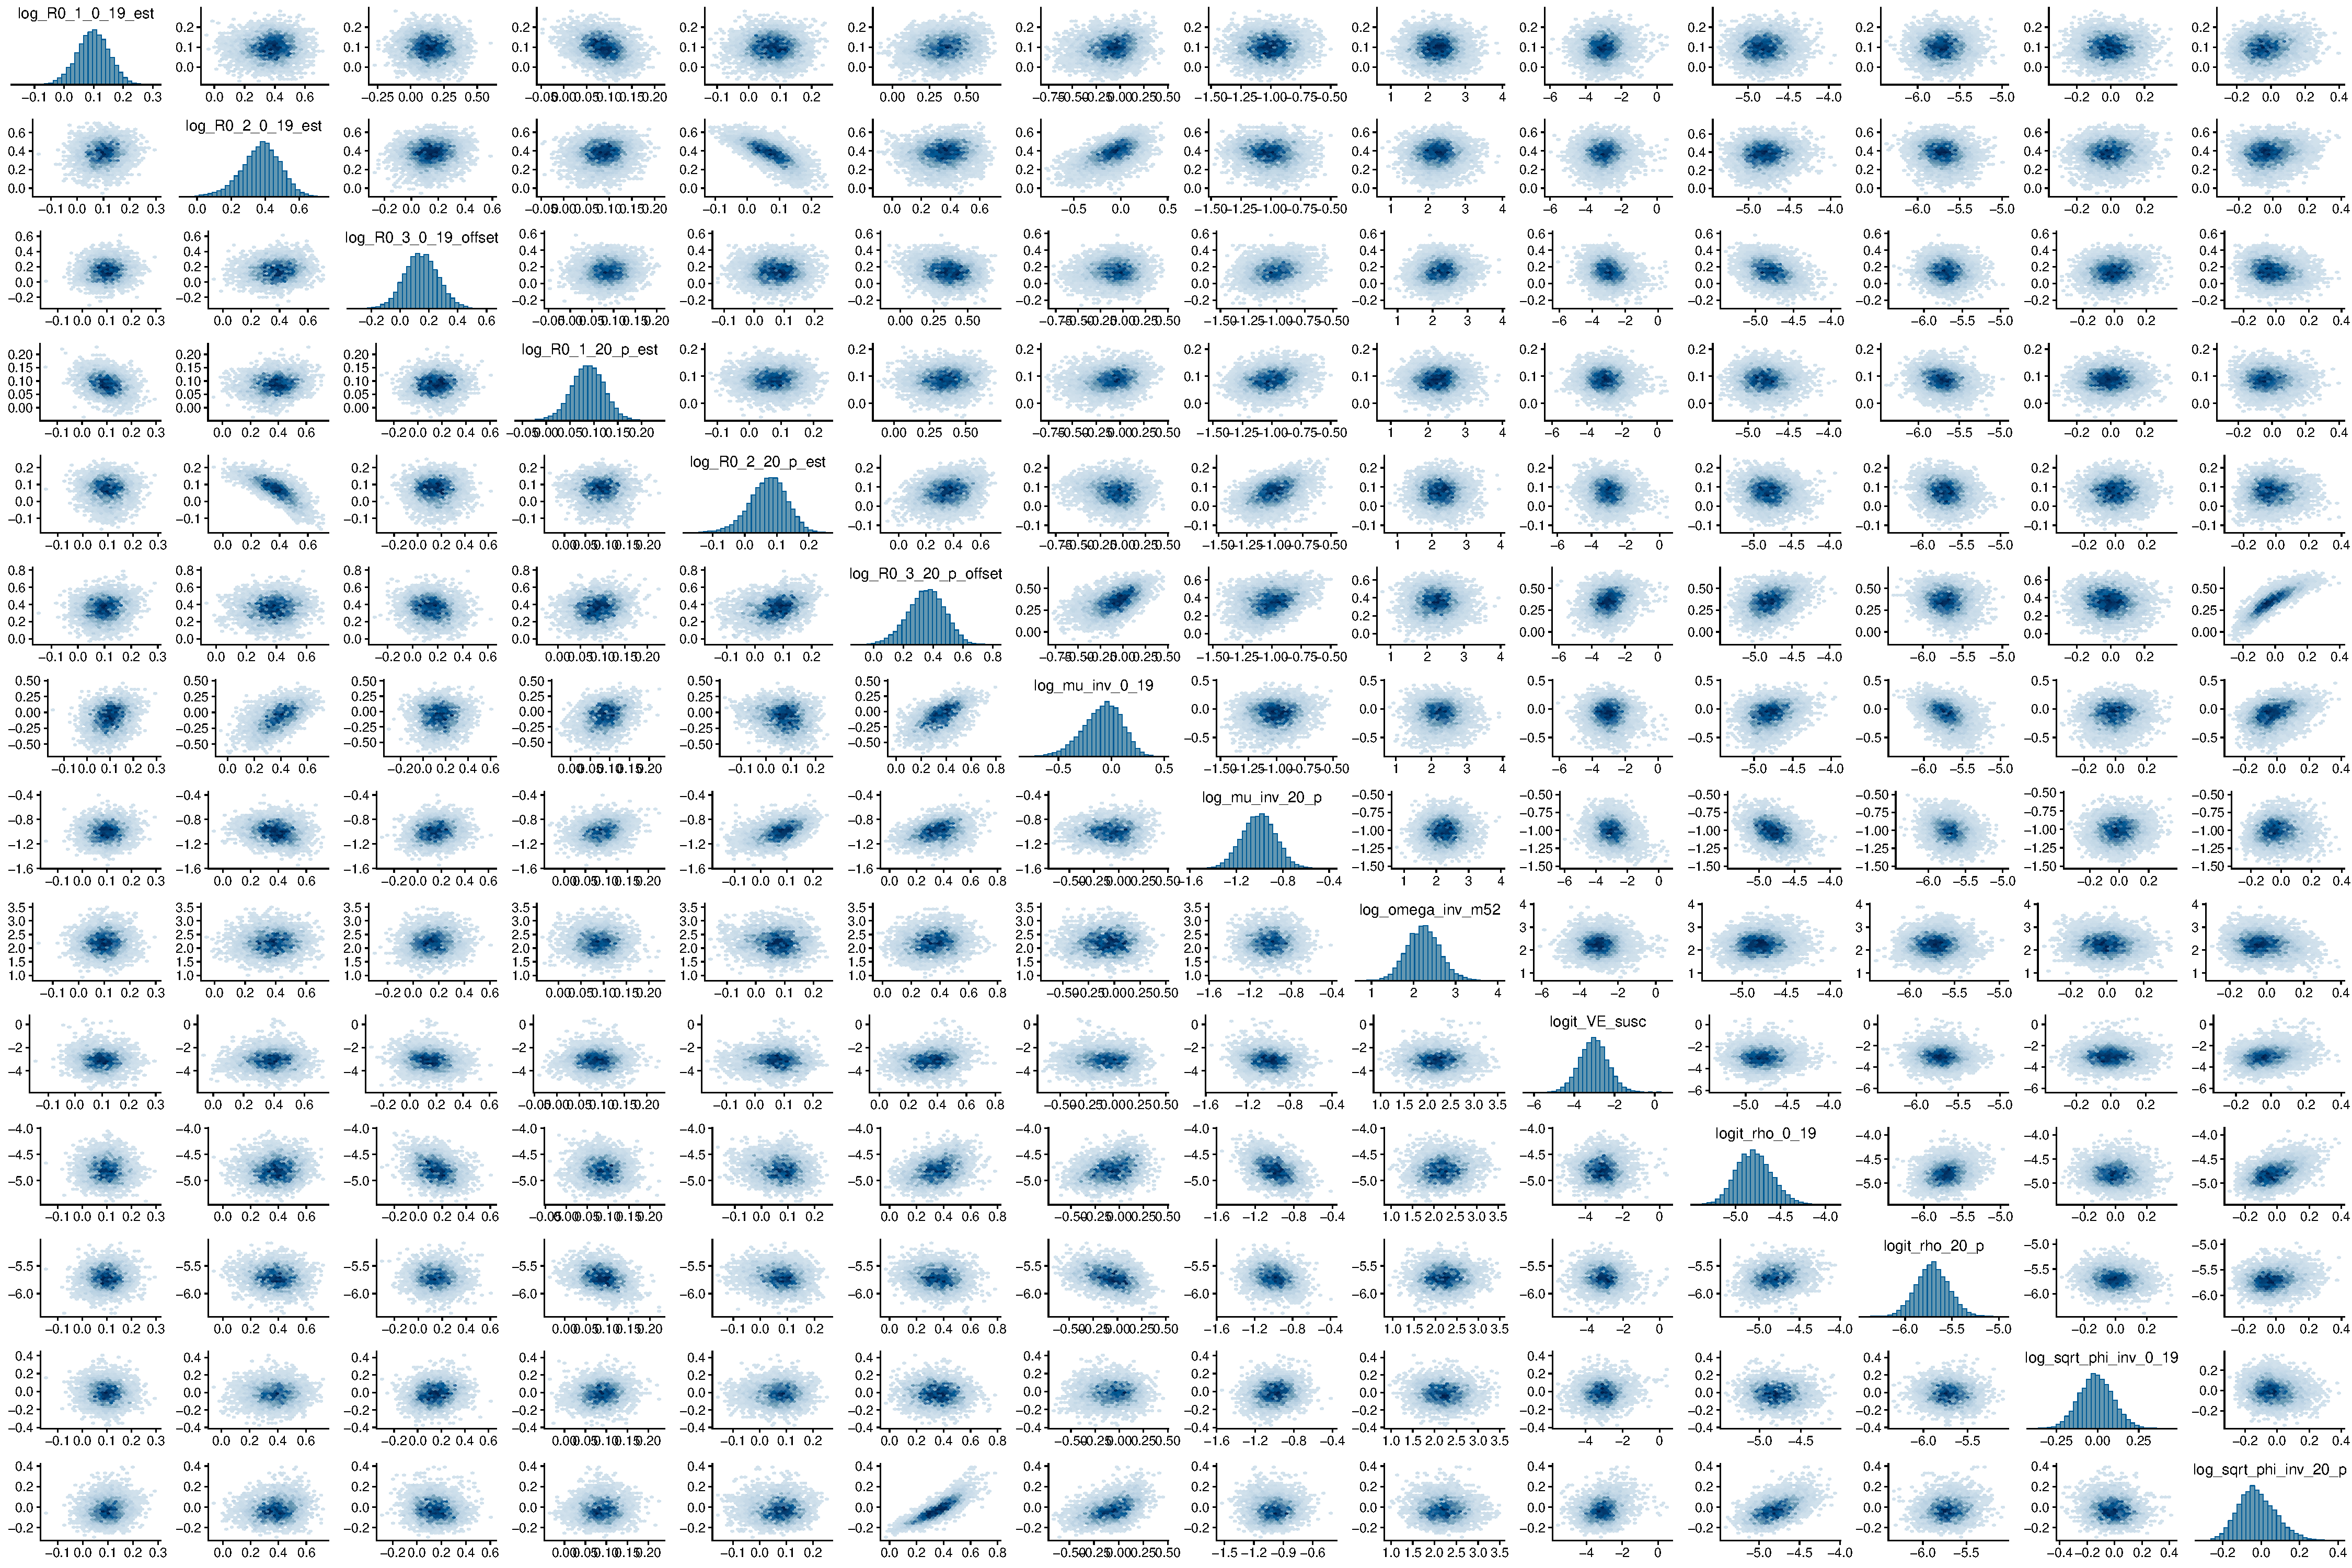
\includegraphics[width=\linewidth]{figures/flu_rw_pairs}
	\caption{Histograms and pairwise scatterplots of posterior samples for the parameters of a stratified SIRS ODE model with time varying dynamics that were sampled via MVNSS. The model was fit to data from the A(H1N1) influenza pandemic in Finland.}
	\label{fig:flurwpairs}
\end{sidewaysfigure}

\newpage

\subsubsection{Stratified SIRS model with piecewise--homogeneous dynamics}
\label{subsubsec:flu_additional_res_const}

\begin{sidewaystable}[htbp]
	\begin{fullpage}
		\caption[Parameters and priors for age--vaccination stratified piecewise homogeneous SIRS ODE models fit to the A(H1N1)pdm09 influenza outbreak in Finland.]{Parameters and priors for age--vaccination stratified piecewise homogeneous SIRS ODE models fit to the A(H1N1)pdm09 influenza outbreak in Finland, prior distributions used in the main analysis. Vaccination adjusted intrinsic reproduction numbers are defined as in equation (\ref{eqn:R0_adj}).}
		\label{tab:flu_priors_const}
		\scriptsize
		\centering
		\begin{tabular}{lllrr}
			\hline
			\textbf{Parameter} &  \textbf{Interpretation} & \textbf{Prior} & \textbf{Median (95\% Interval)} & \textbf{References} \\ \hline
			$ \log(\psi^{adj}_{Y,0}) $ & Intrinsic reproduction \# & $N$(log(1.05), $ 0.025^2 $) & $ \psi^{adj}_{Y,0} = 1.05\ (1.00, 1.09) $ & Nearly endemic dynamics \\ 
			$ \log(\psi^{adj}_{Y,19}) $ & Intrinsic reproduction \# & $N$(log(1.075), $ 0.03^2 $) & $ \psi^{adj}_{Y,19} = 1.075\ (1.00, 1.09) $ & Nearly endemic and $ \psi^{adj}_{Y,19} > \psi^{adj}_{Y,0} $ \\ 
			$ \log(\psi^{adj}_{Y,71}) $ & Adjusted intrinsic reproduction \# & $N$(log(1.2), $ 0.06^2 $) & $ \psi^{adj}_{Y,71} = 1.2\ (1.09, 1.32) $ & Nearly endemic with 10\% immune \\ 
			$ \log(\psi^{adj}_{A,0}) $ & Intrinsic reproduction \# & $N$(log(1.05), $ 0.025^2 $) & $ \psi^{adj}_{A,0} = 1.05\ (1.00, 1.09) $ & Nearly endemic dynamics \\ 
			$ \log(\psi^{adj}_{A,19}) $ & Intrinsic reproduction \# & $N$(log(1.075), $ 0.03^2 $) & $ \psi^{adj}_{A,19} = 1.075\ (1.00, 1.09) $ & Nearly endemic and $ \psi^{adj}_{A,19} > \psi^{adj}_{A,0} $ \\ 
			$ \log(\psi^{adj}_{A,71}) $ & Adjusted intrinsic reproduction \# & $N$(log(1.3), $ 0.07^2 $) & $ \psi^{adj}_{A,71}= 1.3\ (1.16, 1.46) $ & Nearly endemic w/ 10\% immune, $ \psi^{adj}_{A,71} > \psi^{adj}_{Y,71} $ \\
			$ 7/\mu_{Y}-1 $ & Avg. infectious period, youths (days--1) & $N$(0.41, 0.32$ ^2 $) & $  7/\mu_Y =$ 2.5 (1.9, 3.55) & \cite{biggerstaff2014estimates,carrat2008time,cori2012estimating,vink2014serial}\\
			$ 7/\mu_A -1 $ & Avg. infectious period, adults (days--1) & $N$(0.22, 0.165$ ^2 $) & $ 7/\mu_A =$ 2.25 (1.95, 2.63) & $ 1/\mu_Y > 1/\mu_A $,  \cite{biggerstaff2014estimates,carrat2008time,cori2012estimating,vink2014serial}\\
			$ \log(52/\omega) $ & Mean duration of immunity (years) & $N$(1.1, 0.3$ ^2 $) & $ 52/\omega = 3 $ (1.8, 4.9) & $ \Pr(\text{Lose immunity in 1 year}) = 0.3 $ \\
			$ \logit(\nu) $ & 1 - VE for susceptibility & $N$(-1.39, 1) & $ \nu = 0.2\ (0.05,\ 0.56) $ & \cite{lansbury2017effectiveness,syrjanen2014effectiveness}\\
			$ \logit(\rho_Y) $ & Mean case detection rate, youths & $ N(\logit(0.0125),\ 0.31^2) $& $ \rho = 0.0125\ (0.0075,\ 0.02) $ & \cite{shubin2016revealing}\\
			$ \logit(\rho_A) $ & Mean case detection rate, adults & $ N(\logit(0.01),\ 0.31^2) $& $ \rho = 0.01\ (0.006,\ 0.017) $ & $ \rho_A < \rho_Y $, \cite{shubin2016revealing}\\
			$ \log(1/\sqrt{\phi_Y}) $ & Neg. binom. overdispersion, youths & $ \exp(1) $ & 0.69 (0.05, 3.0) & It works.\\
			$ \log(1/\sqrt{\phi_A}) $ & Neg. binom. overdispersion, adults & $ \exp(1) $ & 0.69 (0.05, 3.0) & It works.\\
			\hline
		\end{tabular}
	\end{fullpage}
\end{sidewaystable}

\begin{sidewaysfigure}[htbp]
	\centering
	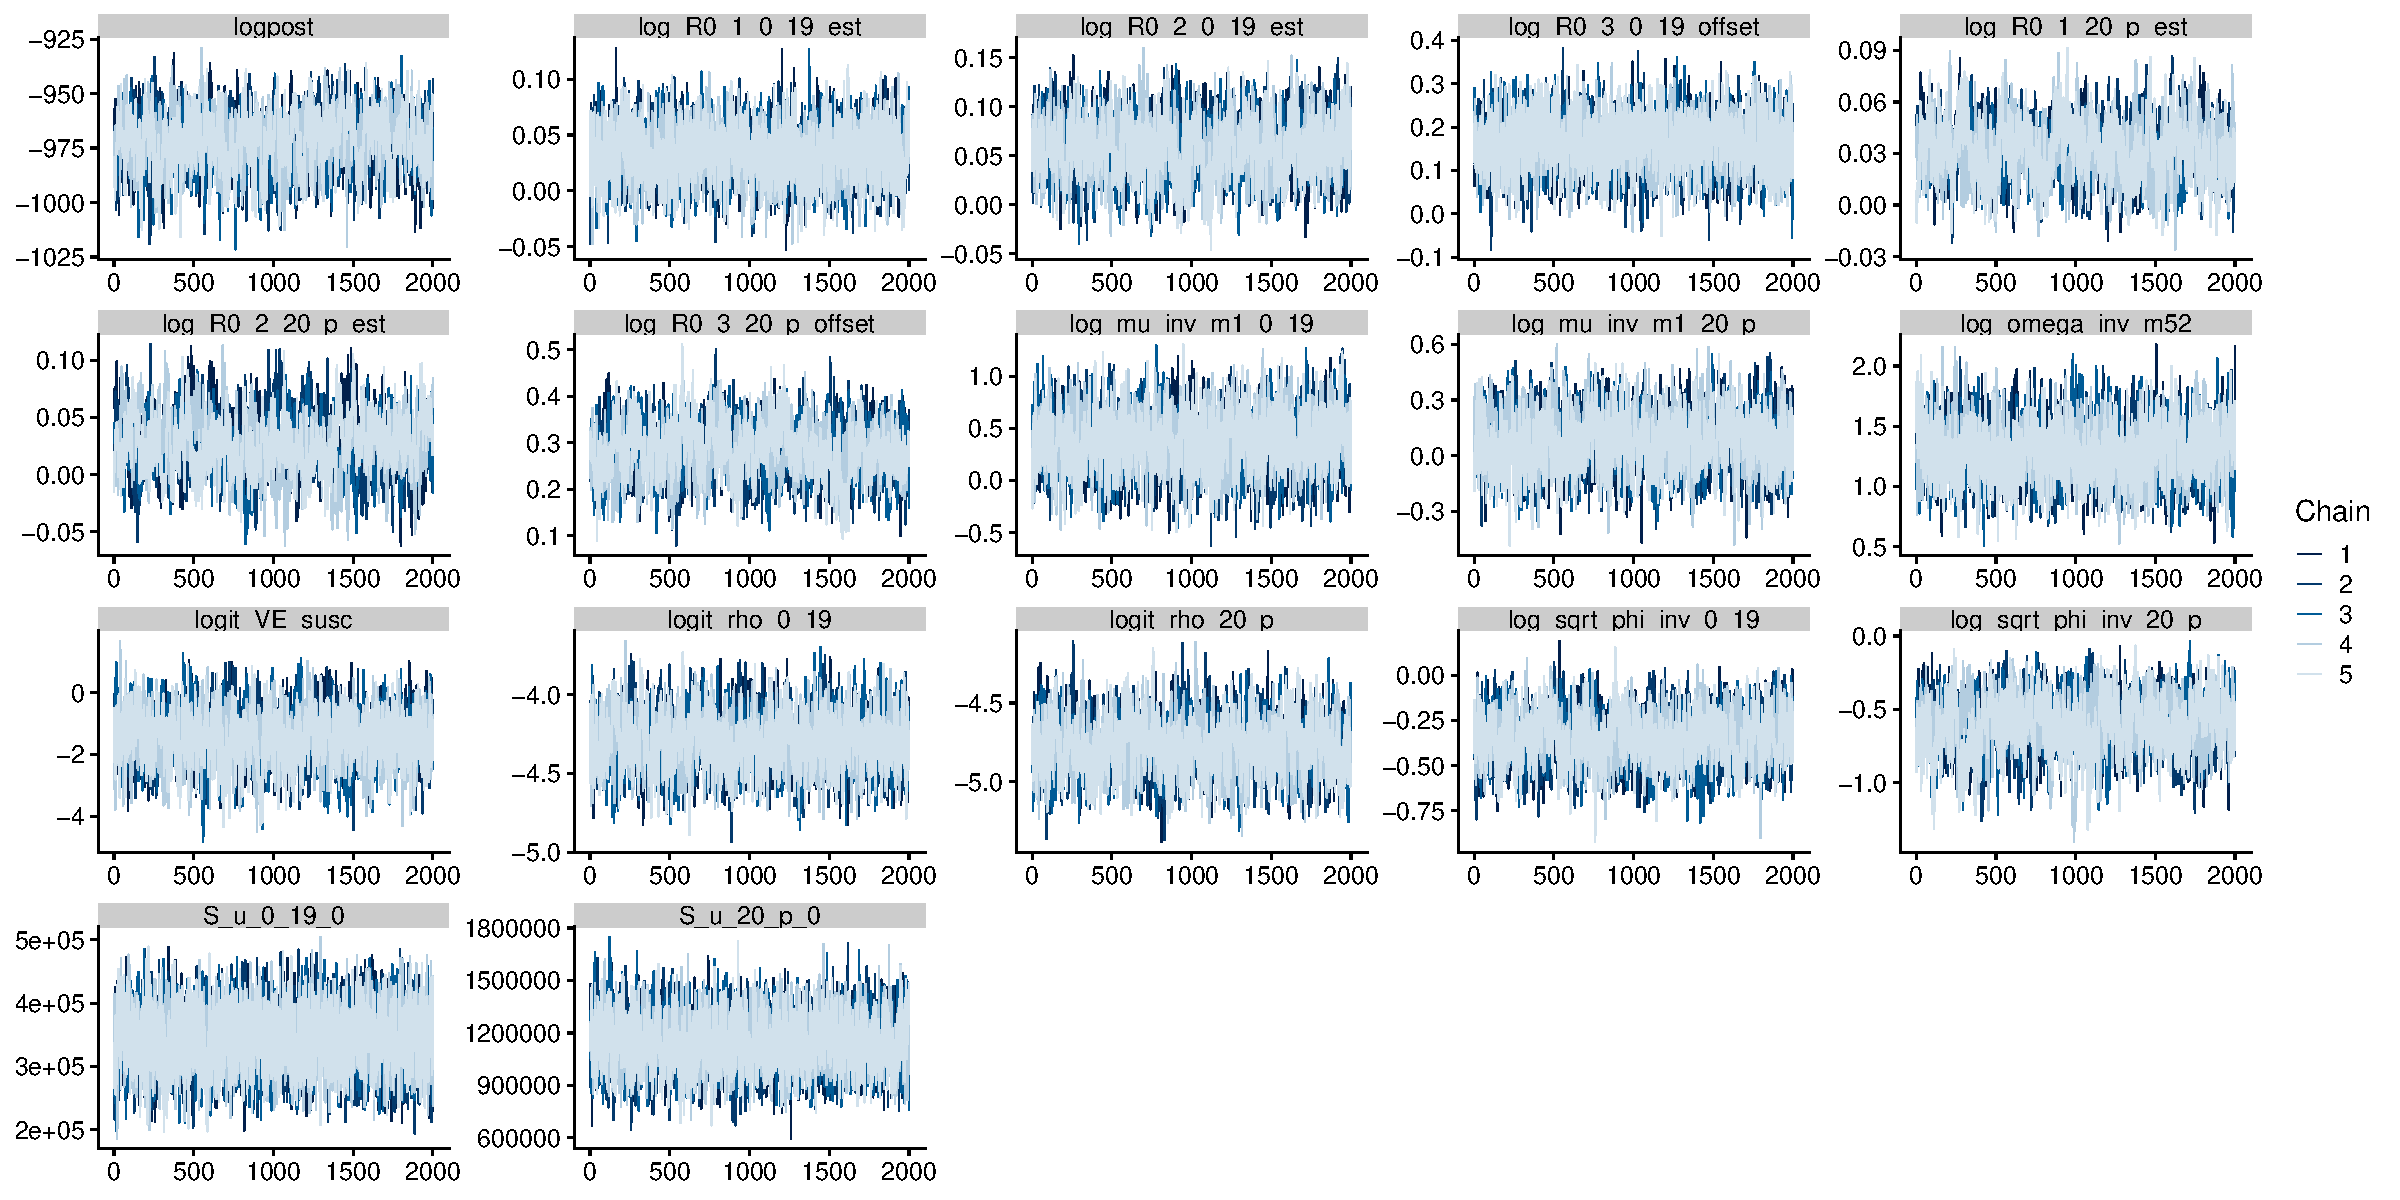
\includegraphics[width=\linewidth]{figures/flu_traces_const_ode}
	\caption{Posterior traceplots for a stratified SIRS ODE model with piecewise--homogeneous dynamics fit to data from the A(H1N1) influenza pandemic in Finland.}
	\label{fig:fluconstodetraces}
\end{sidewaysfigure}


\begin{sidewaysfigure}[htbp]
	\centering
	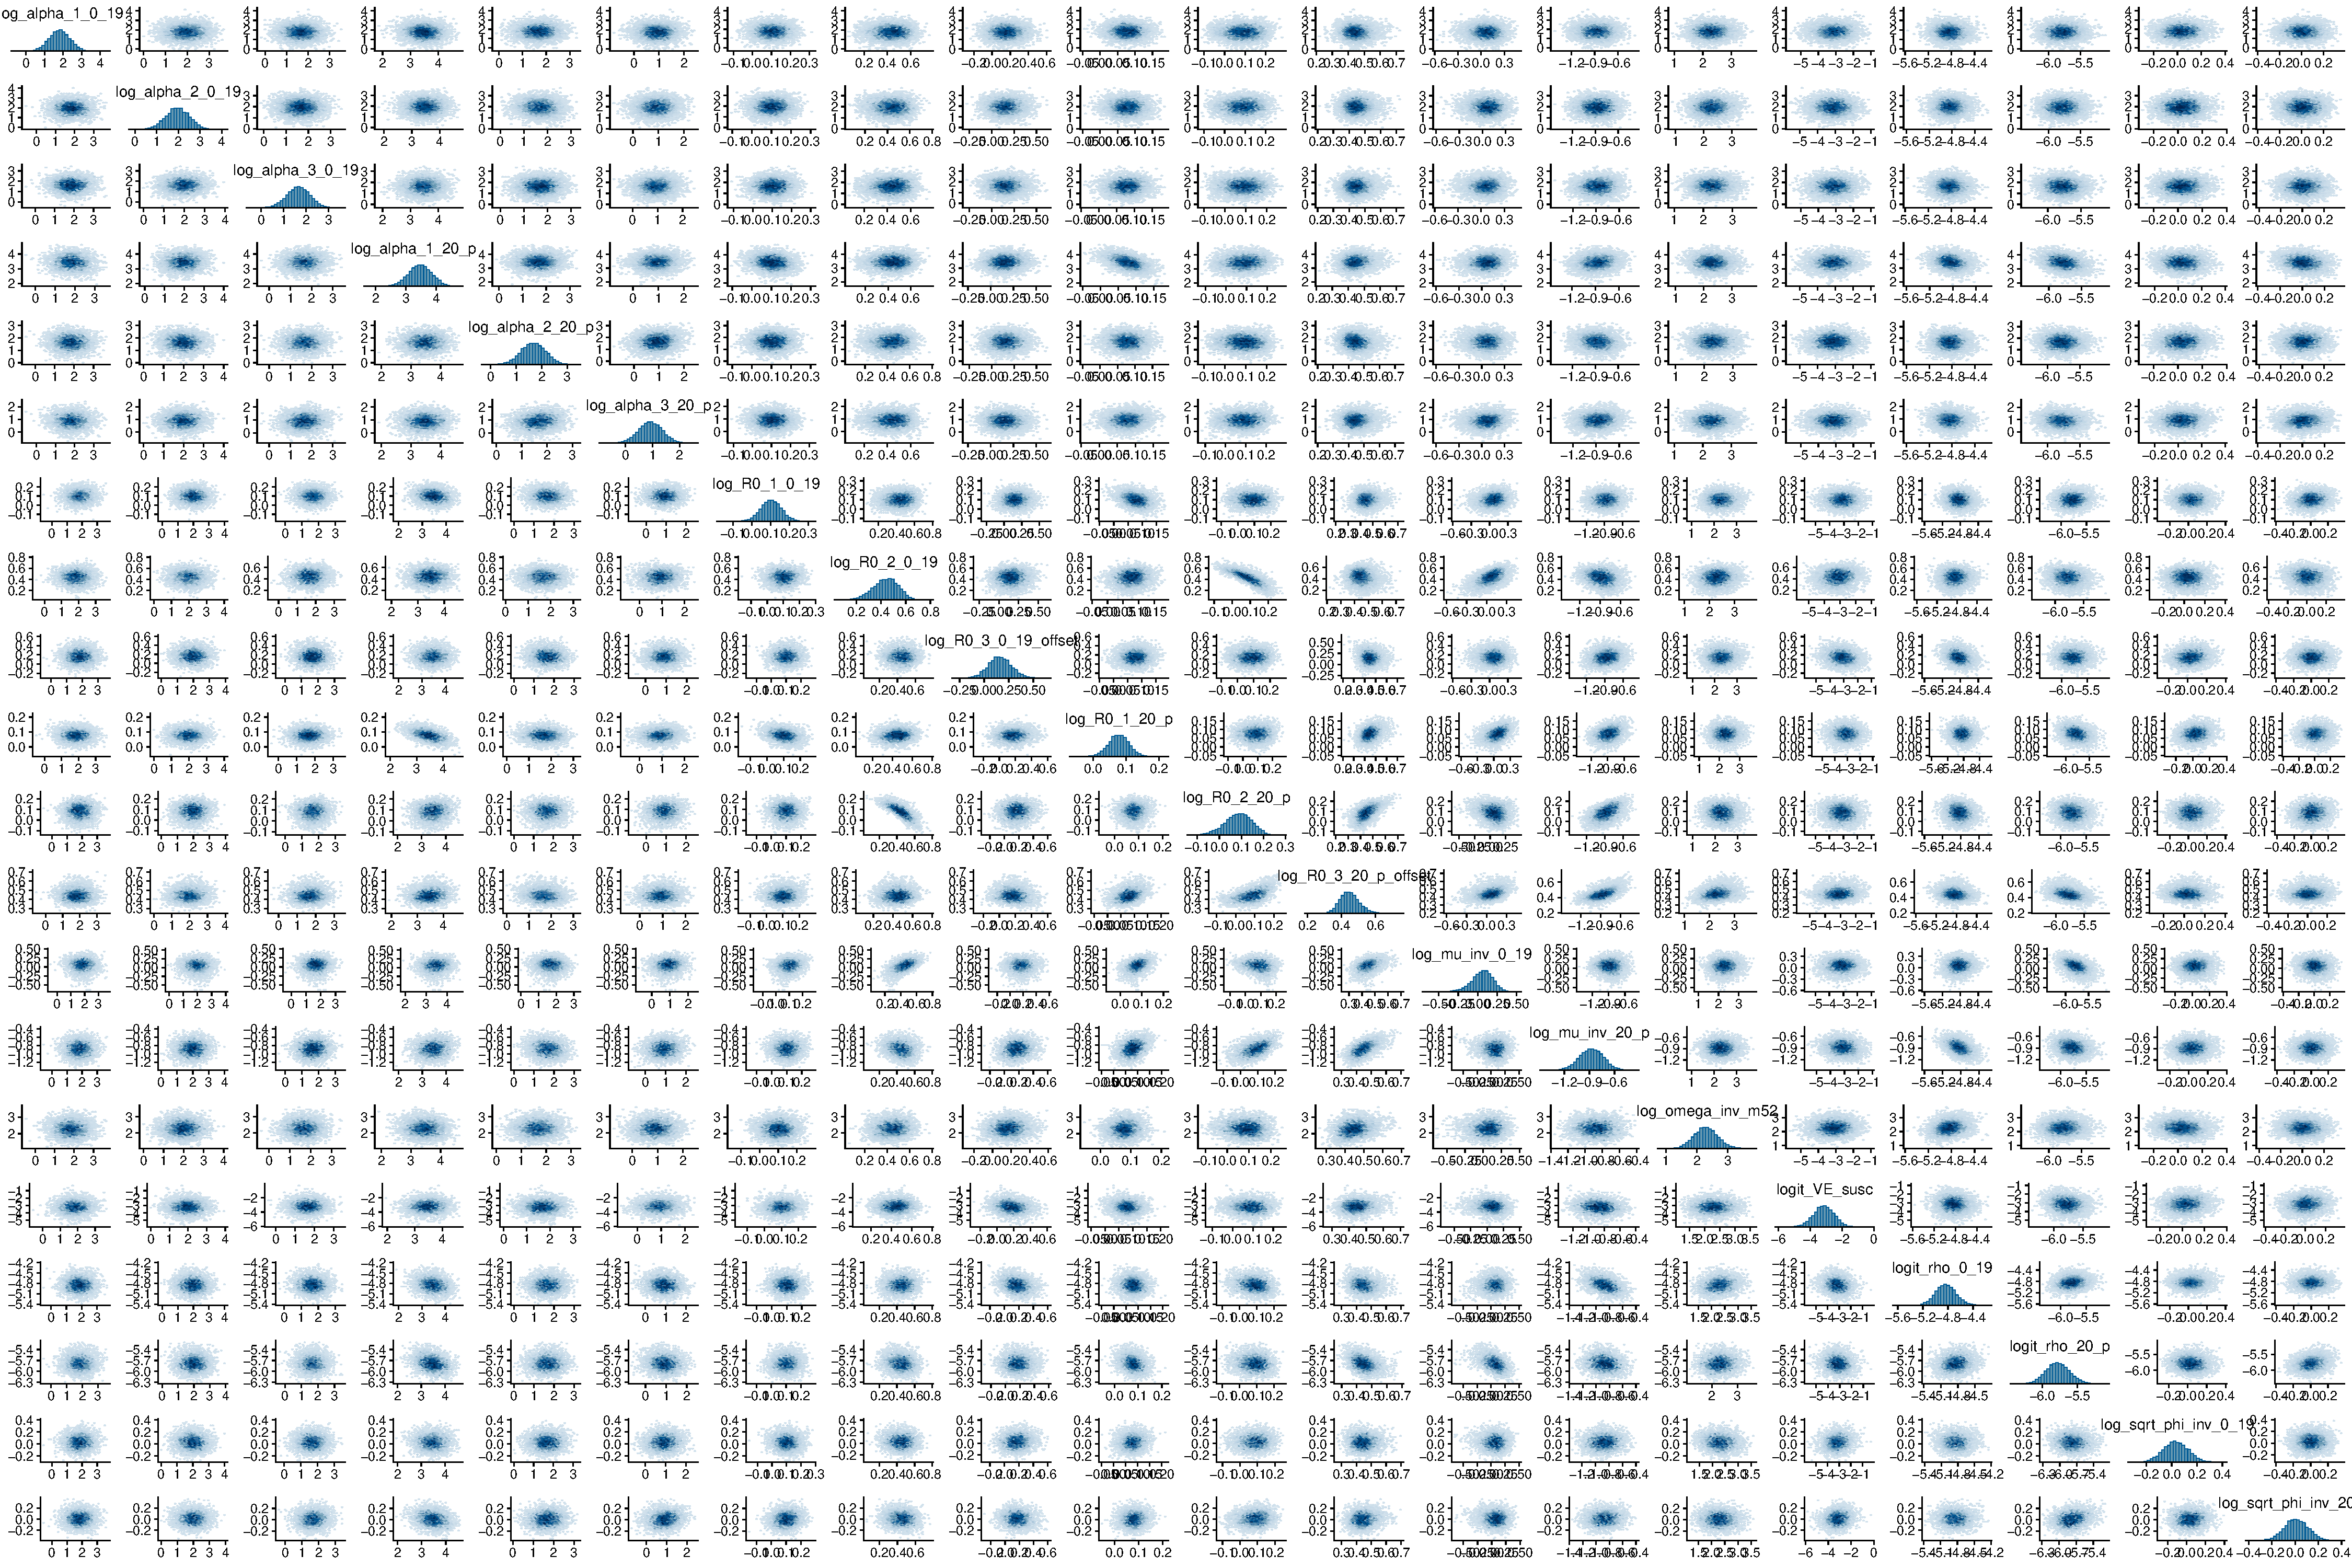
\includegraphics[width=\linewidth]{figures/flu_const_pairs}
	\caption{Histograms and pairwise scatterplots of posterior samples for the parameters of a stratified SIRS ODE model with piecewise homogeneous dynamics that were sampled via MVNSS. The model was fit to data from the A(H1N1) influenza pandemic in Finland.}
	\label{fig:fluconstpairs}
\end{sidewaysfigure}

\newpage
\subsection{Sensitivity to Distribution of Initial Numbers of Susceptibles}
\label{subsec:flu_highsusc_sensitivity}

We fit a supplementary model to explore the sensitivity of estimates of model parameters and incidence to the prior for the susceptible fraction of each age stratum. We again used a multivariate normal approximation to a dirichlet--multinomial distribution for the initial distribution of individuals. The hyperparameter for youths was $$ \balpha_Y = ({S_{Y,0}^{(u)}} = 25, {I_{Y,0}^{(u)}}=0,{R_{Y,0}^{(u)}}=0,D_{Y,0}^{(v)} = 25), $$ so that 50\% of youths were initially susceptible, with the central 80\% of the prior mass between 40\% and 60\%. The hyperparameter for adults was $$ \balpha_A = ({S_{A,0}^{(u)}} = 20, {I_{A,0}^{(u)}}=0,{R_{A,0}^{(u)}}=0,D_{A,0}^{(v)} = 60), $$ so that 25\% of each stratum was initially susceptible, with the central 80\% of the prior mass between 19\% and 31\%. The other priors and various aspects of the model and MCMC were otherwise the same as in the main model with time varying dynamics.

The effect of centering the prior for the fraction of youths who were susceptible, but roughly holding constant the fraction of susceptible adults (the prior in the sensitivity analysis was slightly more diffuse), is that attack rates among youths are inflated, while attack rates among adults are largely similar (Table \ref{tab:flu_attack_rates_sensitivity}). Estimates of the rate parameters governing the model dynamics are largely unchanged from estimates from the main analysis (Table \ref{tab:flu_param_ests_sensitivity}). However, we find that the detection rate among youths is meaningfully lower than the estimated mean case detection rate in the main analysis, which is unsurprising since the estimated incidence is higher. The corresponding estimates for adults are essentially unchanged. In both analyses, the estimated susceptible fractions of each age stratum essentially recover the prior. This suggests that there is not enough signal in the partially observed incidence data to disentangle the effective population size and detection rate. 


\begin{sidewaystable}[htbp]
	\caption[Estimated A(H1N1) infections and attack rates by season and age stratum.]{Estimated infections (thousands) and attack rates by season and age stratum. Attack rates are calculated as the number of infections divided by the size of each stratum, assuming that cases are unique.}
	\label{tab:flu_attack_rates_sensitivity}
	\centering\footnotesize
	\begin{tabular}{lrrrrrr}
		\hline
		&\multicolumn{6}{c}{\textbf{Main analysis}}\\
		\cmidrule{2-7} & \multicolumn{2}{c}{\textit{Season 1}} & \multicolumn{2}{c}{\textit{Season 2}} & \multicolumn{2}{c}{\textit{Both Seasons}}\\
		\cmidrule(r){2-3}\cmidrule(lr){4-5}\cmidrule(l){6-7} & 
		Incidence ($ \times10^3 $) & Attack rate (\%) & Incidence ($ \times10^3 $)& Attack rate (\%) & Incidence ($ \times10^3 $) & Attack rate (\%)\\
		\hline
		Ages 0-19 & 174 (127, 231) & 14.2 (10.4, 18.9) & 68.6 (46.6, 100) & 5.6 (3.8, 8.2) & 244 (181, 321) & 19.9 (14.8, 26.2)\\
		Ages 20+ & 356 (243, 501) & 8.6 (5.9, 12.1) & 171 (117, 245) & 4.1 (2.8, 5.9) & 530 (378, 720) & 12.8 (9.2, 17.4)\\
		All ages & 532 (393, 703) & 9.9 (7.4, 13.1) & 240 (172, 333) & 4.5 (3.2, 6.2) & 774 (586, 1,010) & 14.5 (11, 18.8)\\
		\hline &&&&&&\\
		&\multicolumn{6}{c}{\textbf{Higher susceptible \%}}\\
		\cmidrule{2-7}	& \multicolumn{2}{c}{\textit{Season 1}} & \multicolumn{2}{c}{\textit{Season 2}} & \multicolumn{2}{c}{\textit{Both Seasons}}\\
		\cmidrule(r){2-3}\cmidrule(lr){4-5}\cmidrule(l){6-7} & 
		Incidence ($ \times10^3 $) & Attack rate (\%)& Incidence ($ \times10^3 $) & Attack rate (\%)& Incidence ($ \times10^3 $) & Attack rate (\%)\\
		\hline
		Ages 0-19 & 281 (198, 384) & 23 (16.2, 31.4) & 95.2 (66, 141) & 7.8 (5.4, 11.5) & 377 (276, 502) & 30.9 (22.6, 41)\\
		Ages 20+ & 349 (232, 496) & 8.4 (5.6, 12) & 175 (119, 251) & 4.2 (2.9, 6.1) & 526 (367, 717) & 12.7 (8.9, 17.4)\\
		All ages & 632 (470, 823) & 11.8 (8.8, 15.4) & 272 (193, 374) & 5.1 (3.6, 7) & 907 (689, 1,170) & 16.9 (12.9, 21.8)\\
		\hline
	\end{tabular}
\end{sidewaystable}


\begin{sidewaystable}[htbp]
	\caption[Posterior estimates of SIRS model parameters for pandemic A(H1N1) influenza in Finland --- Sensitivity analysis to prior distribution for the effective population size.]{Posterior estimates of SIRS model parameters from the main analysis compared to estimates obtained with a higher number of susceptible youths. Estimated posterior medians (95\% Bayesian credible intervals).} 
	\label{tab:flu_param_ests_sensitivity}
	\centering\footnotesize
	\begin{tabular}{clrr}
		\hline
		&&\multicolumn{2}{c}{\textbf{Dynamics}}\\
		\cmidrule{3-4}\textbf{Parameter} & \textbf{Interpretation} & \textit{Main analysis} & \textit{Higher susceptible \%}\\
		\hline
		$ \psi_{Y,0} $ & Intrinsic $ R_0 $ for youths at epiweek 15, 2009  & 1 (0.99, 1.1) & 1 (0.99, 1.1)\\
		$ \psi_{Y,19} $ & Intrinsic $ R_0 $ for youths at epiweek 35, 2009 & 1.1 (1, 1.1) & 1.1 (1, 1.1)\\
		$ \psi_{Y,71}^{adj} $ & Vaccination adjusted intrinsic $ R_0 $ for youths at epiweek 33, 2010 & 1.2 (1, 1.3) & 1.2 (1, 1.3)\\
		$ \psi_{A,0} $ & Intrinsic $ R_0 $ for adults at epiweek 15, 2009  & 1 (1, 1.1) & 1 (1, 1.1)\\
		$ \psi_{A,19} $ & Intrinsic $ R_0 $ for adults at epiweek 35, 2009 & 1 (0.98, 1.1) & 1 (0.97, 1.1)\\
		$ \psi_{A,71}^adj $ & Vaccination adjusted intrinsic $ R_0 $ for adults at epiweek 33, 2010 & 1.3 (1.2, 1.5) & 1.3 (1.2, 1.5)\\
		$ 1/\mu_{Y} $ & Mean infectious period for youths (days) & 2.5 (1.9, 3.5) & 2.3 (1.8, 3.1)\\
		$ 1/\mu_A $ & Mean infectious period for adults (days) & 2.1 (1.8, 2.4) & 2.1 (1.8, 2.5)\\
		$ 1/\omega $ & Mean duration of immunity (years) & 3.6 (2.4, 5.8) & 3.6 (2.4, 5.8)\\
		$ \nu $ & 1 - VE for susceptibility & 0.19 (0.039, 0.54) & 0.17 (0.036, 0.5)\\
		$ s_Y $ & \% susceptible youths, $ S^{(u)}_Y(t_0) / N_Y $ & 0.28 (0.21, 0.36) & 0.5 (0.38, 0.63)\\
		$ s_A $ & \% susceptible adults, $ S_A^{(u)}(t_0) / N_A $ & 0.28 (0.21, 0.35) & 0.28 (0.21, 0.36)\\
		$ \rho_Y $ & Mean case detection rate for youths & 0.013 (0.0097, 0.019) & 0.0099 (0.0072, 0.013)\\
		$ \rho_A $ & Mean case detection rate for adults & 0.0084 (0.0061, 0.012) & 0.0081 (0.006, 0.011)\\		
		$ 1/\sqrt{\phi_Y} $ & Negative binomial overdispersion for youths & 0.71 (0.55, 0.92) & 0.65 (0.5, 0.86)\\
		$ 1/\sqrt{\phi_A} $ & Negative binomial overdispersion for adults & 0.56 (0.37, 0.76) & 0.54 (0.38, 0.74)\\
		\hline
	\end{tabular}
\end{sidewaystable}